\chapter{Enhancing Process-Based Models for Precision Soil Moisture Forecasting}
\label{physics-aware-chap:orchard}

The possibility to accurately and precisely forecast agricultural systems can provide significant improvement in a variety of agricultural issues such as irrigation demand, drought, climate change, nutrient depletion, and soil degradation \cite{vitali2021crop}.
Agronomists leverage well-accepted and solid process-based models, specifically crop models such as CRITERIA \cite{Bittelli2011253} and HYDRUS \cite{hydrus2008587}.
A crop model describes the growth and development (phenology from germination to harvest) of a crop, at the level of the field, the canopy, and the plant (Goudriaan and van Laar 1994).
In doing so, a limited number of primary physiological and physical processes (e.g., surface runoff, deep percolation, soil evaporation and plant transpiration) are estimated using differential equations, climate data and crop-specific input parameters.
Outputs of one process can serve as input to other processes, and so on and so forth, computing a series of time steps until the output of the final analysis is returned.
The overall computation is called \textit{simulation}; for instance, in our case of soil moisture forecasting in kiwifruit, our proposed crop model simulates soil moisture dynamics across the whole irrigation season, in each soil unit, until the desired horizon is reached.

\begin{figure}[t]
	\centering
	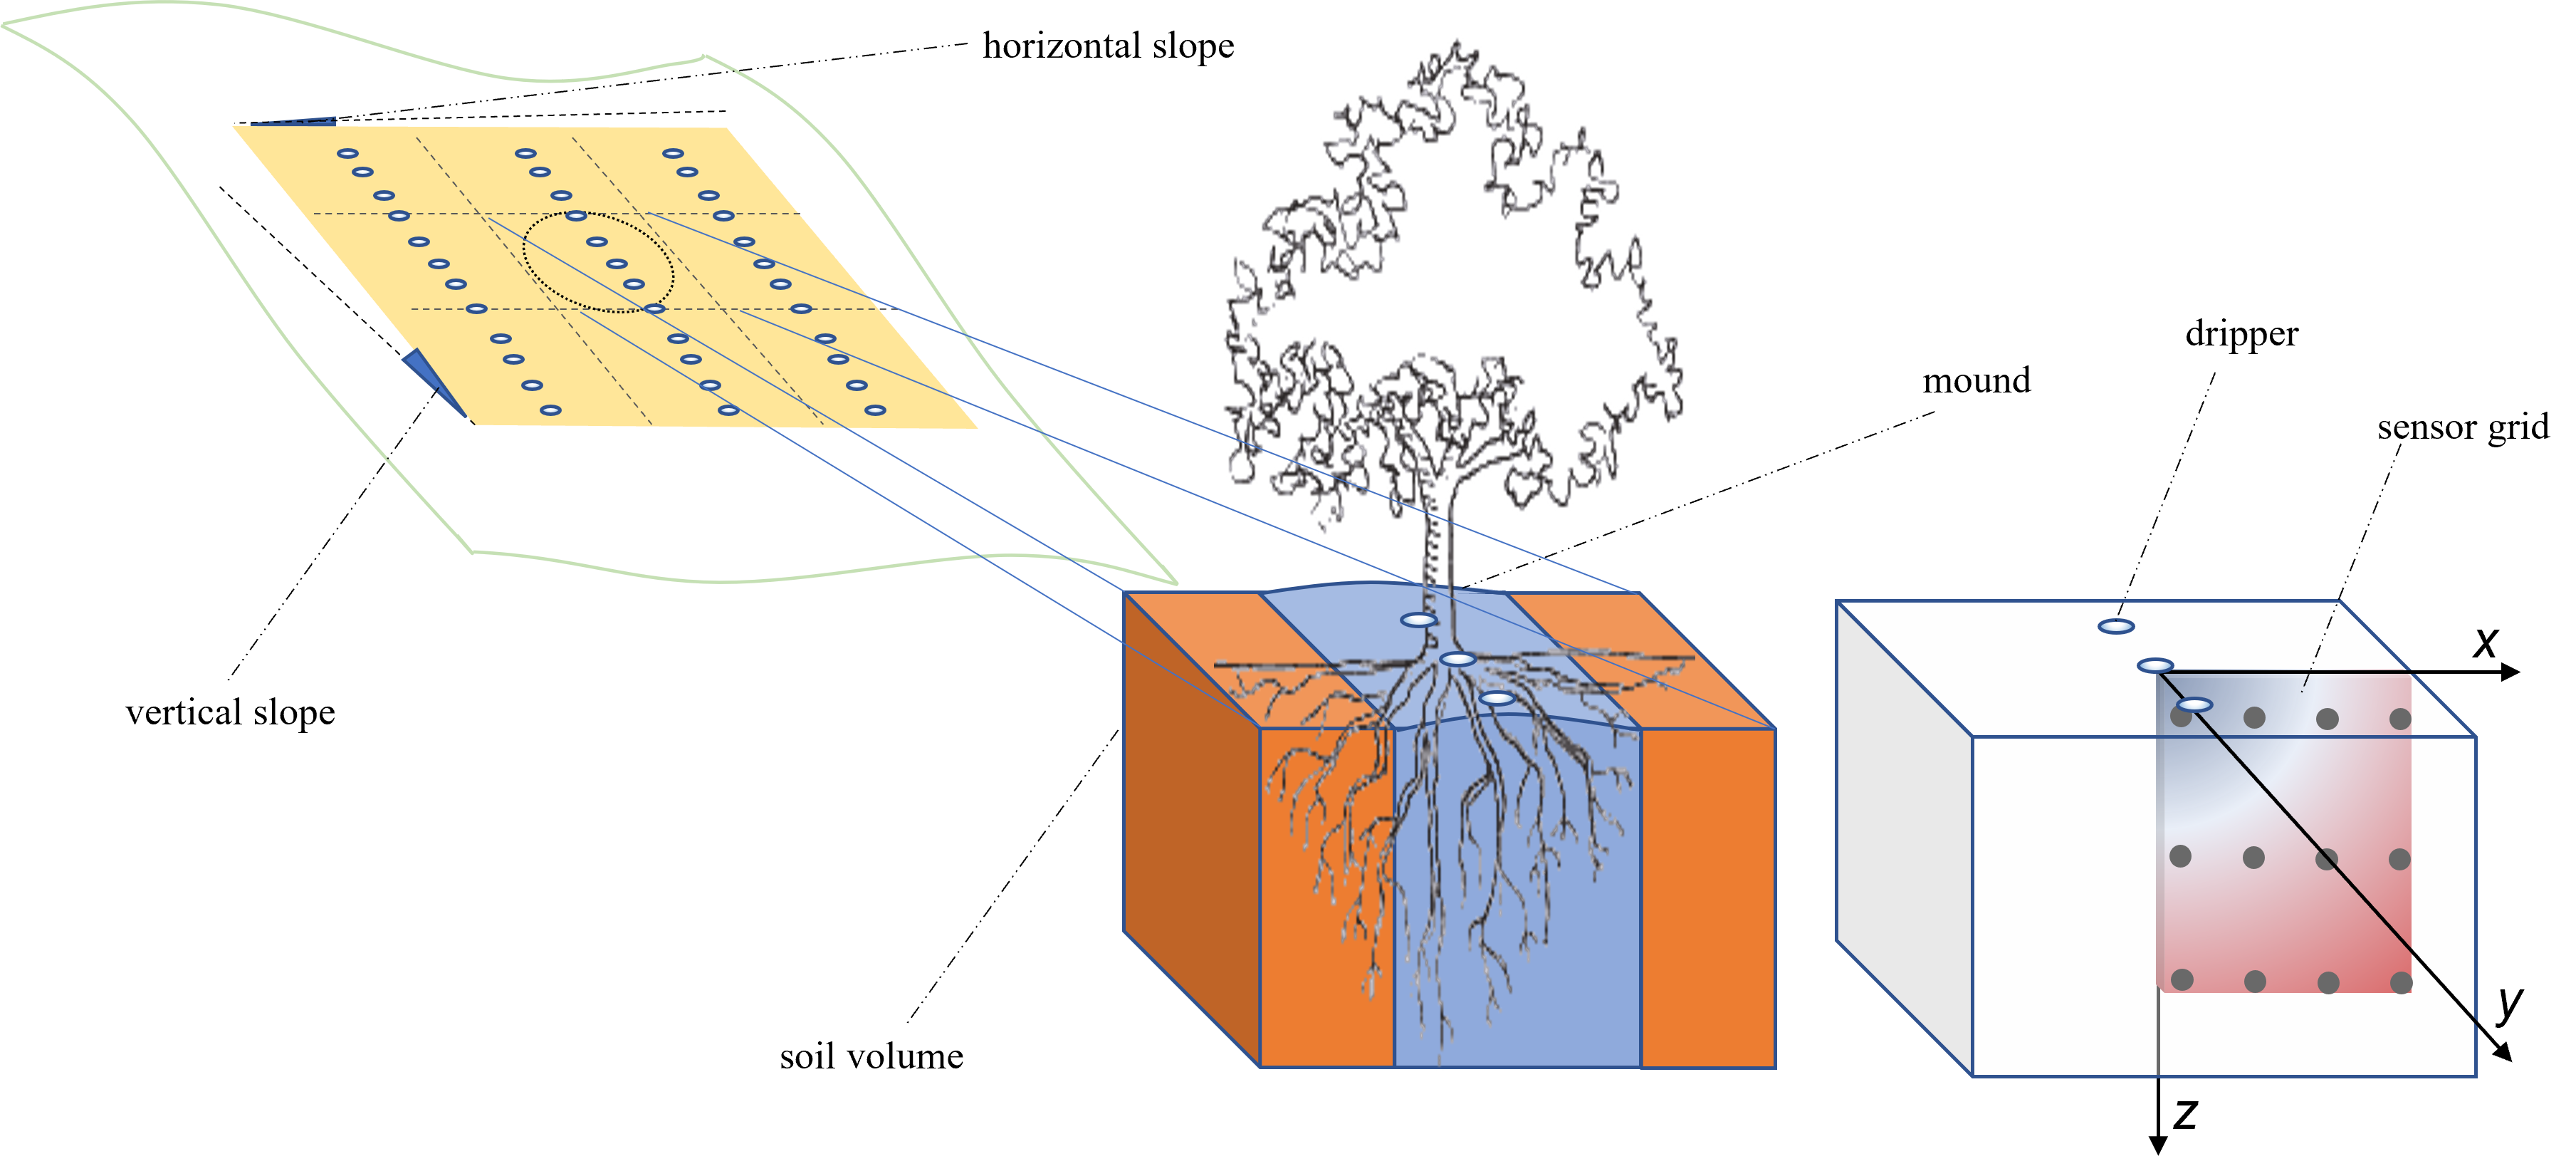
\includegraphics[scale=0.5]{chapters/physics-aware/orchard/img/OverallPlantingLayout3.png}
	\caption{Schematic depicting the planting layout (inter- and intra-row distances).}
	\label{orchard-fig:scheme1}
\end{figure}

\paragraph{Challenges} \cite{silva-giller-2020} presented a series of relevant questions regarding the ability of such crop models to address several issues.
First, the authors stressed the importance of coupling models with in-situ data for an effective application at the operational level---i.e., \textit{data assimilation}.
% The uncertainty associated with crop modeling computation can be reduced by coupling these models with real-time measurements relevant to the soil and crop.
Today, with digitalization and remote acquisition of real-time data, it is possible to effectively incorporate experimental data and modeling in a real-time framework.
Second, crop models imply the measurement of a variety parameters---such as soil texture, leaf are index (LAI), water table  \cite{marshall-etal-1996}.
Measurement of all these variables is usually not feasible for operational conditions in real-world farms, therefore tiuning such simulation parameters play a fundamental role.
Finally, many crops are still under-represented in crop models, including tropical perennials and fruit trees.
Among fruit trees, the kiwifruit (\emph{Actinidia deliciosa}) has been only partially studied, not enough to precisely quantify its water demands.
% The kiwifruit -- often shortened to kiwi (used hereafter) -- is an edible fruit that originated in China and got widely diffused in many countries.
% Italy is the third largest producer of kiwi worldwide, with a yearly production of 524,490 MTons \cite{fao-2020}.
% Since it originated in areas with large availability of water (central and eastern China), this plant has high water demand.
% In the Emilia-Romagna region (Italy), the kiwi irrigation season generally starts in May and ends in October \cite{villani-etal-2011}, with high water demands in a period where droughts and water scarcity are becoming more frequent due to climate change.
% While these effects of climate change also apply to other countries \cite{olesen-etal-2011}, worldwide temperature increases and precipitations decrease \cite{ec-2013}, having adverse impacts on agriculture \cite{bindi-olensen-2011}.
% In a study on irrigation demand projections in kiwi, \cite{villani-etal-2011}
% reported that for the 2021-2050 period, wrt. the 1961-1990 period, a general
% increase of more than 10\% is expected.

% Authors reported average daily evapotranspiration for kiwi ranging from 62 to 80 m$^3$ day$^{-1}$ in New Zealand, while \cite{judd-etal-86} showed a water consumption ranging from 80 and 103 m$^3$ day$^{-1}$ in the central zone of South America \cite{valenzuela-88}. According to \cite{judd-etal-86} the high
% water demand is due to the large leaf-surface area and low stomata control. \cite{xiloyannis-etal-90} recommended to keep the soil water
% content at levels higher than 50 \% of the degree of saturation
% for optimal yield. Due to these high water consumptions kiwi is commonly an irrigated crop in most of the areas where it is cultivated such as New Zealand \cite{hall-etal-2001}, Chile \cite{holzapfel-etal-2000} and Italy \cite{xiloyannis-etal-90}.

% Few research papers have been published on measuring and modeling kiwi water demand. Indeed, in a review on fruit tree crop models, \cite{grisafi-etal-2021} showed that only one research was published on modeling kiwi and with emphasis on carbon budget, but not on the soil water budget. Little has also been done in terms of modeling the plant's water use and transpiration. \cite{rallo-etal-2020} presented a review about FAO56 crop coefficients of fruit trees and vines, performed over the past twenty years, to update information and extend tabulated single and basal standard crop coefficients. Also in this review it appears that kiwi is highly under-represented with only one listed research by \cite{silva-etal-2008}, where kiwi's transpiration was measured with a sap flow method.

% The high water consumption of kiwi has raised concerns about groundwater depletion and it has fostered interest in developing increasingly efficient irrigation systems and scheduling to optimize water use. For instance, if excess irrigation water is applied, water resources are mismanaged with additional costs including energy to activate water pumps, leaching of mobile fertilizers (nitrates) into the groundwater and potential for soil erosion; on the other hand, if the soil is water depleted from lack of adequate irrigation, plant production may be reduced with financial costs for the farmers.

To mitigate water wasting, soil moisture forecasting is used to correctly plan irrigations.
Predictions must rely on a robust crop model able to compute the water budget---i.e., estimate soil water requirement, in the root zone, to keep the cultivated plant in optimal conditions.
% This implies the measurement and/or the computation of a variety of processes including surface runoff, deep percolation into the groundwater, capillary rise from the groundwater, subsurface lateral flow, soil evaporation and plant transpiration \cite{marshall-etal-1996}.
% Measurement of all these variables is usually not feasible for operational conditions in real-world farms, therefore  play a fundamental role along with measurements of weather data and a few, key soil variables.
% Weather data can be easily provided with low cost portable weather stations, or by downloading data from weather data networks.
% Weather forecast is provided by local public agencies or by private companies. It is not difficult today to obtain a relatively low cost service for weather forecasting. Soil properties such as SWC and SWP are easily measured by installing low cost sensors in the soil profile \cite{bittelli-2010,nagahage-etal-2019}.


%DATA ASSIMILATION
% The challenging aspect for a correct simulation of the water budget is the parameterization and corroboration of the simulation model. Parameterization can be obtained from experimental determination of soil and plant properties. For instance, the soil hydraulic properties (the soil water retention and hydraulic conductivity curves) can be measured in the laboratory.
% However, these measurements are expensive and time-consuming. It is rarely a feasible solution for farmers, to measure the soil hydraulic properties.
% An alternative solution is to install soil sensors measuring SWC or SWP and calibrate the model through a process of data assimilation, providing weather and basic soil properties data as input. Key soil variables such as SWC and SWP can be successfully used to asses the water budget computation and plant water requirements.

% Data assimilation is a very powerful technique even during the forecasting process, since it allows to initialize each simulation with the real soil state, thus to a low error state. In real-case problems, there are no error-free estimations and many slight errors gradually lead the model to progressively deviate especially for domains in which a wide range of different phenomena interacts. In particular, soil moisture forecasts are affected by weather forecasts (influenced in turn by plenty of variables), water tables, soil slopes, hysteresis, and so on.

% Today many companies commercialize affordable and reliable sensors to be installed in orchards. In our approach we exploit a grid of sensors rather than a single one. This makes it possible to create a precise map of the water content that, in turn, increases data assimilation accuracy.

\paragraph{Contributions}
In this chapter, we propose \olab: a crop model enhanced with data assimilation and auto-tuning techniques.
Specifically, we commit to the following contributions.
\begin{itemize}
	\item An innovative \textit{3D crop model} designed specifically to compute the soil water balance of an orchard.
    The 3D model keeps into account: non uniform distribution of the root system, growth and development of orchard plants with a full computation of the soil water budget, short-term weather forecast.
    \item A \textit{data assimilation} technique to map coarse-grained 2D/3D-sensor grid to the fine-grained 3D moisture profile, leveraged as a checkpoint state for the crop model.
    \item A \textit{parameter tuning} to automatically calibrate the model parameters to a specific orchard borrowing AutoML techniques---i.e., Bayesian (hyper)parameter optimization.
	\item A detailed field experiment in a kiwifruit field in a commercial farm.
\end{itemize}


\begin{figure}[t]
	\centering
	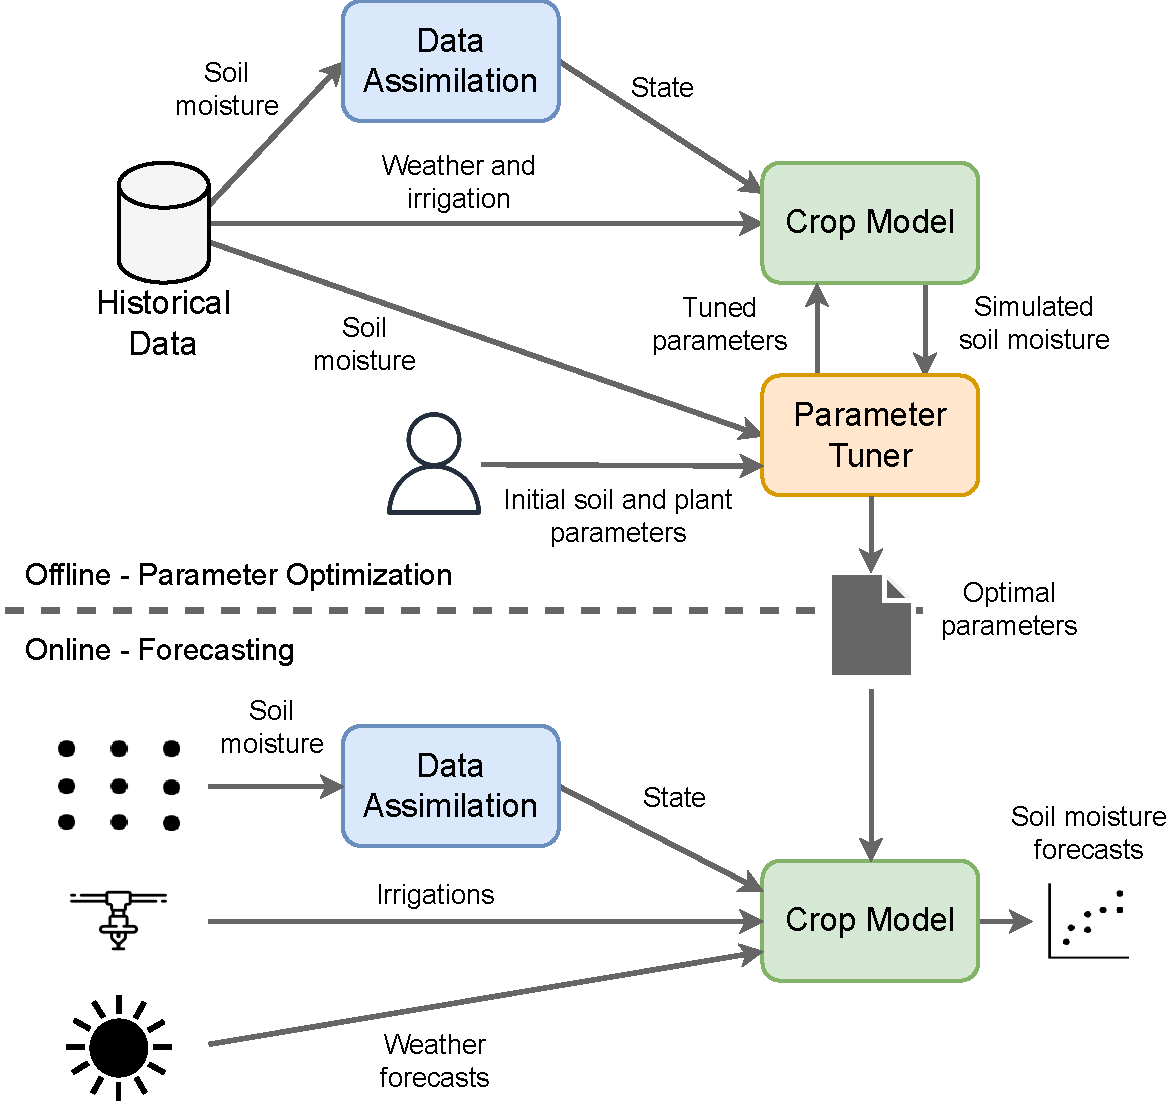
\includegraphics[width=0.75\textwidth]{chapters/physics-aware/orchard/img/overview.pdf}
	\caption{Approach overview and main system components.}
	\label{orchard-fig:overview}
\end{figure}


\section{Orchard3D-Lab}

\Cref{orchard-fig:scheme1} depicts the planting layout adopted.
 Trees are arranged in lines; soil can have a slope both in the $x$ and $y$ axes. The orchard is equipped with a watering system that can be of different type (e.g., single or double wing) and with different distances between drippers and lines. For each plant, we consider a \emph{soil volume} that includes the roots; typically the soil volume can be larger than the area affected by the watering system. A mound can be present to favor draining.

The simulation approach and the required functional modules are depicted in \Cref{orchard-fig:overview}. The offline phase is aimed at determining the optimal crop model parameters. The \emph{parameter tuner} searches for the best parameters by comparing data simulated by the crop model with the \emph{Historical Data} from real sensors.
Historical data must cover the time period of the simulation scenario, including watering and weather conditions (typically obtained from in-situ weather stations or from public open data) together with their effect on soil water content (i.e., the values sampled by soil sensors).

The online phase requires the grid of sensors to be in place. During this phase the crop model, properly set with the optimal parameters, forecasts the system behavior and exploit the \emph{data assimilation} module to initialize the simulation model to the real field status.


\Cref{tab:parameter} shows the simulation parameters: in bold those automatically inferable by the tuning phase, while the remaining ones must be provided by the user. Note that, if no historical values are available tuning cannot be run. In this case the on-line phase will be based on default values possibly taken from the literature. Similarly, if some of the tunable parameters are known, tuning can be limited to the remaining ones.

The following subsections describe in more details each of the components reported in \Cref{orchard-fig:overview}.

\begin{table}[t]
	\centering
	\scriptsize
	\begin{tabular}{p{1.2cm}p{5cm}p{7.5cm}}
 		\textbf{Type} & \textbf{Parameter} & \textbf{Description} \\
		% \multicolumn{1}{p{2cm}}{\textbf{Type}} & \textbf{Parameter} & \multicolumn{1}{p{2cm}}{\textbf{Description}} \\
		\hline%\midrule
		Field & Location &  Latitude, longitude and altitude $[m]$ of the field\\
		& Slopes & Slopes $[m \cdot m^{-1}]$ of the simulated field \\
		& Mound & Slope $[m \cdot m^{-1}]$ and width $[m]$ of the mound \\
		& \textbf{Water table} $\in [1.5..5]$ & Depth $[m]$ of a aquifer\\ 
		\hline%\midrule
		\multirow{2}{1cm}{Soil Layer*} & Thickness & Thickness $[m]$ of the soil layer moved from Domain\\
		& Texture & Portion of sand, silt and clay $[\%]$ \\ % esiste mappa dei suoli in regione
		& \textbf{Ksat $\in [10^{-7}..10^{-3}]$ } & Saturated hydraulic conductivity  \\ % valore di default da soil editor (fitting non lineare, oppure fitting lineare con un ordine +/- rispetto a valore di default). Da convertire da cm/gg a m/s
		& $\pmb{\theta_s}$ $\in [0.2..0.7]$ & Saturated water content $[-]$\\  
		& $\pmb{\theta_r}$ $\in [0.02..0.7]$ & Residual water content $[-]$ \\  
		& $\pmb{\alpha}$ $\in [0.5..5]$ & Modified Van Genuchten inverse air entry suction $[m^{-1}]$\\  
		& $\mathbf{n}$ $\in [1..2]$ & Modified Van Genuchten pore-size distribution\\
		& \textbf{he $\in [0..15]$} & Modified VanGenuchten/Campbell air mat. pot. $[m H_2O]$ \\ 
		& \textbf{b} $\in [1..9]$ & Campbell empirical retention parameter\\ 
		\hline%\midrule
		Plant* & Position & Position $[m]$ of the plant(s) in the domain area\\
		& \textbf{Radius} $\in [1..3]$ & Radius $[m]$ of the canopy \\
		& \textbf{Leaf area index} $\in [3..5]$ & Green leaf area per unit ground surface area\\ % se distribuzione delle piante uniforme (i.e., molto vicine), possiamo tenerlo fisso
		& \textbf{Roots depth} $\in [0.5..1.2]$ &  Origin and maximum depth $[m]$ of roots\\
		& \textbf{Roots deformations} $\in [0..2]$ &  Root deformation factors on x and z axes\\ 
		& \textbf{Kc max} $\in [0.8..4]$ &  Maximum crop coefficient\\
		& \textbf{fRAW} $\in [0...1]$ & Readily available water fraction\\
		\hline%\midrule
		\multirow{2}{1cm}{Irrigation elem*} & Type & Irrigation type of the element(s) \\
		& Position & Position of the element(s)\\
		\hline%\midrule		
		Model & Geometry  & Length $\times$ width $\times$ depth $[m]$ of the simulated field\\
		& Cell size  &  Size $[m]$ of a single parallelepipeds simulation unit\\% having parallelepipeds geometry. \\ % Size $[m]$ of a single simulation unit having parallelepipeds geometry.
% 		& Boundary conditions $\in [free\_drainage, default]$ & \textcolor{orange}{Description needed}\\ 
		& Ret. curve $\in [Camp., mod Van Genuc.]$ & Water retention model\\ 
  		% & Retention curve $\in [Campbell, modified Van Genuchten]$ & Water retention model\\ 
	    & Conduct. mean $\in [log, harm, geom]$ &  Water conductivity averaging method \\ % Conductivity
		& \textbf{Conductivity H/V Ratio} $\in [0..1]$  &  Water conductivity horizontal/vertical ratio \\
		\bottomrule
	\end{tabular}%
	\begin{tablenotes}
      \scriptsize
      \item Types with * can have several elements. Parameters in bold are targeted by the parameter tuning.
    \end{tablenotes}
	\caption{System parameters.}
	\label{tab:parameter}%
\end{table}%

\subsection{The Crop Model}

\newcommand{\Wt}{$\overrightarrow{W}$}
\newcommand{\It}{$\overrightarrow{I}$}
\newcommand{\SMt}{$\overrightarrow{SM}$}

We propose an innovative model specifically devised for computing the soil water budget in an orchard.
The solution is based on the integrated finite difference (also called cell-centered finite volume scheme) method.
The crop model builds on \textit{Criteria-3D} \cite{bittelli-etal-2015} and introduces the following features in the computation of the soil water budget in an orchard:
\begin{itemize}
 \item a fully coupled three-dimensional model of the soil water budget;
    \item a plant growth model for the orchard tree is included, including root's system and calibration of tree parameters described in \Cref{orchard-sec:evapotrans} and \Cref{orchard-sec:root};
    \item application of the three-dimensional computation specifically for an orchard with land slopes and drip irrigation system;
    \item data assimilation from a sensor grid.
\end{itemize}


The crop model accounts for saturated water flow, unsaturated water flow, and surface runoff and it is coupled with a model for soil evaporation and plant water uptake. The soil moisture state is stored as a 3D-matrix ($SM$): each cell of the matrix represents a portion of the soil volume along with its simulated soil moisture.

\Cref{alg:ocrchad3d-lab} describes how a simulation is implemented: from an assimilated state, through an iterative process that computes the soil moisture given the time series of weather and irrigation data.

\begin{algorithm}[t]
\caption{Crop Model}
% \footnotesize
\begin{algorithmic}[1]
\Require{$SM_{Ass}$: assimilated soil moisture, \Wt: weather time series, \It: irrigation time series, X: parameters from \Cref{tab:parameter}} 
\Ensure{\SMt: time series of simulated soil moisture}
    \State $SM_0 \gets SM_{Ass}$ \Comment{Initialize the simulator state}
    \State \SMt $\gets [~]$ \Comment{Initialize the accumulator}
    \ForEach{$t \in$ \Wt, \It} \Comment{For each timestamp...}
        \State $SM_{t+1} \gets  Richards(w_t, i_t, SM_t)$ \Comment{... calculate the next state}
        \State \SMt $\gets$ \SMt $~\frown~(t+1, SM_{t+1})$ \Comment{... append it}
    \EndFor
    \State \Return \SMt \Comment{Return the time series of soil moisture}
\end{algorithmic}
\label{alg:ocrchad3d-lab}
\end{algorithm}

More in details, the crop model takes as inputs the state $SM_{Ass}$ that is computed through data assimilation as in \Cref{orchard-ssec:ass}), a time series of weather conditions at increasing timestamps (\Wt$=[(t, \textup{humidity}, \textup{air temperature}, \textup{solar radiation}, \textup{wind speed}), ...]$), a time series of irrigations at increasing timestamps (\It$=[(t, \textup{irrigation}), ...]$), and the set of parameters $X$ from \Cref{tab:parameter}.
We assume \Wt{} and \It{} to be aligned over time and to be at the same time granularity of the simulation.
First, we initialize the simulator state with the assimilated sensor data (Line 1) and the time series in which the simulated soil moisture will be accumulated (Line 2).
For each timestamp (Line 3), the current weather, irrigation and  simulator state are leveraged to update the state of the simulator using Richards equation (Line 4) and the new state is accumulated (Line 5).
Finally, the time series of soil moisture over the whole period is returned (Line 6).

The crop model solves Richards' equation \cite{richards1931capillary} to compute water flow.
For each cell of soil in our 3D-matrix, it calculates the change of the water potential and volumetric water content in time.
This demands information about: (i) the soil hydraulic properties, (ii) the amount of water to sink (e.g., for the root water uptake), (iii) the boundary conditions (i.e., behavior at the boundary of the soil volume at hand).
In the following, \Cref{orchard-sec:soil_properties} provides the main equations leveraged by the crop model to estimate the soil hydraulic properties; \Cref{orchard-sec:evapotrans} and \Cref{orchard-sec:root} describe how to obtain the root water uptake for each portion of soil by, respectively, calculating the overall volume of water leaked for transpiration and splitting it according to the root system; finally, \Cref{orchard-sec:boundary} delves into the boundary conditions.
% Surface runoff can be activated or de-activated. During the calibration procedure the surface runoff can be de-activated to reduce computation time, but during the operational phase of the modeling and forecasting it must be activated to properly partition the surface fluxes given by precipitation and irrigation.
% The model does not simulate preferential flow, solute transport, and channel flow.
% Preferential flow can be emulated by using ``effective'' soil properties (e.g., increased porosity and hydraulic conductivity), if such data are available.

\subsubsection{Soil Hydraulic Properties}
\label{orchard-sec:soil_properties}
Richards' equation is the solution of the mass balance for water in a soil volume.
A fundamental component in its resolution is the description of the hydraulic properties, namely the soil water retention and the hydraulic conductivity function.

The soil water retention curve maps the soil water potential  (i.e., the driving force for flow) to the soil water content (i.e., the amount of water) and is used to describe the drying process of a particular soil.
For its estimation, the van Genuchten-Mualem model is currently the most widely exploited.
Yet, it has been demonstrated that it can lead to erroneous estimates of the hydraulic conductivity.
For this reason, the crop model employs the modified van Genuchten-Mualem model proposed in \cite{ippisch-etal-2006}, where an air entry value is included in the formulation:
\begin{equation}
\label{ippisch}
S_e(h)=          \left\{ \begin{array}{ll}
\frac{1}{S_c} \left[1+(\alpha h)^n \right]^{-m} &\mbox{if $(h > h_e)$}\\
1                             &\mbox{if $(h \leq h_e)$}
           \end{array}
        \right.
\end{equation}
Given $\alpha$ the inverse air entry suction (i.e., value for which we mark the transition between saturated and unsaturated soil mechanics), $m = 1 - 1/n$ a shape-defining pore parameter derived from the pore-size distribution (depending to soil texture and structure), and $S_c = [1+ (\alpha h_e)^n]^{-m}$ the water saturation at $h_e$ the air-entry potential (i.e., the point at the largest pores which air can enter into the soil); the degree of saturation $S_e$ is defined in relation to the soil water potential $h$.

As to the hydraulic conductivity, it is the ease with which water moves through porous spaces and fractures in soil (e.g., a porous soil is said to have a high hydraulic conductivity if water can readily travel through it).
In other words, the flux density is regulated by the ability of the material to transfer water under a certain gradient.
Given a ``tortuosity'' factor $l$, it is possible to calculate the hydraulic conductivity $K$ in relation to the current degree of saturation $S_e$ as:

\begin{equation}
\label{ippisch2} K(S_e)=          \left\{ \begin{array}{ll}
K_s S_e^l \left[\frac{1-(1-(S_e S_c)^{1/m})^m}{1-(1-S_c^{1/m})^m} \right]^{2} &\mbox{if $(S_e < 1)$}\\
K_s                             &\mbox{if $(S_e \geq 1)$}
           \end{array}
        \right.
\end{equation}

The parameter $K_s$ is the saturated hydraulic conductivity, which represents the ability of the soil to conduct water when all the pores are water-filled. When the soil start to desaturate (drying), the hydraulic conductivity decreases with respect to its value at saturation.
The parameters $m$ and $n$ allows the curve to take different slope and shape in its decreasing values from saturation, again depending on texture and structure. 

\subsubsection{Evaporation and Transpiration}
\label{orchard-sec:evapotrans}
The classic approach to estimate the amount of water transpired by the plant is to: compute the overall potential evapotranspiration and, then, calculate the plant's transpiration based on the plant vigor.

The potential evapotranspiration $ET_0$ is calculated by the Penman-Monteith equation for the typical reference crop \cite{allen-etal-1988}.
% This is computed based on the atmospheric evaporative demand for standard conditions and it depends only on atmospheric conditions.
Given the fraction of intercepted Photosynethetically Active Radiation $fPAR$, and the momentary Turbolence Coefficient $TC$, we can derive (under optimal conditions) the maximum potential transpiration $T_{pot}$ and evaporation $E_{pot}$:
%
\begin{equation}
\label{maxET}
T_{pot} = ET_0 \cdot fPAR \cdot TC
\end{equation}
\begin{equation}
\label{minET}
E_{pot}= ET_0 \cdot (1-fPAR)
\end{equation}
%
The partition of radiation $fPAR$ is defined in relation to the light excitation coefficient $KE$, which is the sum of scattering and absorption by particles and gases and it is a measure of the alteration of radiant energy as it passes through the atmosphere and the Leaf Area Index $LAI$ (i.e., the amount of one-sided green leaves per square inch of ground estimating the plant canopy growth).
The selected value of $KE$ was 0.6 which is an average value for atmospheric conditions in the area.
In turn, $LAI$ varies throughout the year according to the plant vigor; for this reason, $SSD$ (i.e., sum of day degrees accumulated by the plant during the growing season) is leveraged:
%
\begin{equation}
\label{fPARi}
fPAR(SDD) = 1- e^ {-KE \cdot LAI(SDD)}
\end{equation}
\begin{equation}
\label{LAI}
LAI(SDD) = \frac{LAI_{max}-LAI_{min}}{1+e^{(a_{LAI}+b_{LAI}\cdot SDD)}}+ LAI_{min}
\end{equation}
$LAI_{max}$ and $LAI_{min}$ are the maximum and minimun possible $LAI$ values respectively, while $a_{LAI}$ and $b_{LAI}$ are crop dependent parameters. Such $LAI$ parameters can be found in literature, and hence derive its value only from $SSD$.

Finally, the turbolence coefficient $TC$ is dependent to the crop coefficient $Kc(SSD)$, a fraction of the water needed for the reference high-water-use grass crop.
Specifically, $TC$ is the crop coefficient for the mid-season development stage of adequately watered crops \cite{driessen1992land}:
\begin{equation}
\label{TC} TC(SSD) = 1 + (Kc_{Max}-1) \cdot fPAR(SSD)
\end{equation}
$Kc_{Max}$ is the value of the crop coefficient when the plant has the maximum value of LAI \cite{allen-etal-1988}.
Its value is either obtained from the literature of from calibration.



\subsubsection{Root System}
\label{orchard-sec:root}
In \olab{}, the overall potential transpiration $T_{pot}$ is divided among each portion of the soil that contains the root system.
The root uptake in a specific point $actTrans(x,y,z)$ varies according to the respective root density $k_{root}(x,y,z)$.
The greater the density, the greater the portion of $T_{pot}$ that is transpired in that point:
%
\begin{equation}
\label{root1} actTrans(x,y,z) = T_{pot} \cdot k_{root}(x,y,z)
\end{equation}
%
By default, the root shape is the ``taproot''.
Besides being a common tree crops, this is generally assumed in kiwi trees. 
This is customizable according to the following conditions:
\begin{itemize}
    \item along the $x$ axis, the root density varies linearly w.r.t. the distance to the dripper line, a parameter (i.e., $root_x$) allows to set a constant density or to drop it to zero at the inter-row;
    \item along the $y$ axis, the root density is assumed to be constant, this is consistent to the model assumptions of constant water content along the dripper line; 
    \item along the $z$ axis, the root density is non-linear, a parameter (i.e., $root_z$) allows to set higher density either in the upper or lower layers.
\end{itemize}

The values of $root_x$ and $root_z$ can be deduced by the parameter tuner.

\Cref{orchard-fig:root} shows the root density projections on the $xy$ and $xz$  planes.
The parameter values shaping the figure routes are those set in the orchard adopted in our experimentation.
Note how moving further away from the center, where the dripper is located, root density decreases both vertically and horizontally. 

\begin{figure}[t]
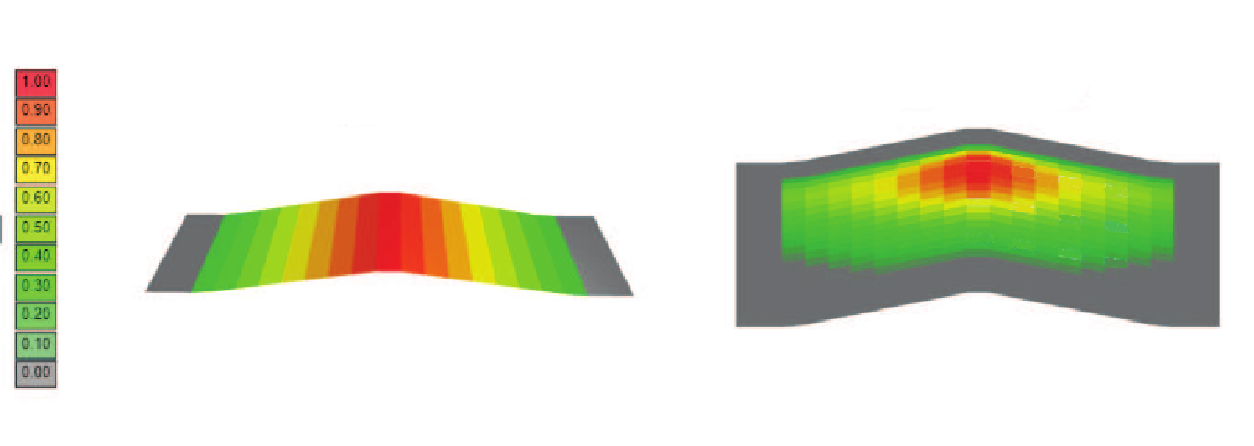
\includegraphics[scale=0.6]{chapters/physics-aware/orchard/img/root.pdf}
\caption{Root schematic: variation of the root density on the $xy$ plane (on the left) and on the $xz$ plane (on the right).}
\label{orchard-fig:root}
\end{figure}


\subsubsection{Boundary Conditions}
\label{orchard-sec:boundary}
To numerically solve the partial differential equations governing Richards water flow, boundary conditions are used to reduce the number of unknown variables.
In practise, we define the behavior of the soil at the boundaries of the simulated volume so that we can determine the solution of the equation (i.e., the value of the flux) in the part of interest.
To properly solve the problem, the boundary conditions should represent the actual conditions of the experiment and, hence, be chosen upon the available information (in this regard, details can be found in \cite{bittelli-etal-2015}). 

\olab{} allows to set up Dirichlet and Neumann boundary conditions.
The former defines the specific value that the flux needs to take along the boundary, the latter defines the desired derivative.
As to Dirichlet boundary conditions, we implemented: nodes (i.e., portions of soils) with fixed hydraulic head (i.e., fixed water potential), and nodes with prescribed flux (i.e., fixed source/sink phenomena). 
The water table is a simple example of nodes with fixed hydraulic head; when this is present, the water potential is set to zero at the water table depth. 
Atmospheric boundary conditions are examples of nodes with prescribed flux.
Positive fluxes are assigned to the surface for either precipitation or irrigation events, negative fluxes to the upper soil layers and rooting depth for potential evapotranspiration.
As to Neumann boundary conditions, the model implements free drainage at the boundaries as a bottom outflow.
The gradient is determined based on the elevation difference among computational nodes,
with the first node in a position outside the computational domain. 

\subsection{Data Assimilation}\label{orchard-ssec:ass}

\begin{figure}[t]
\centering
\begin{subfigure}[t]{.3\textwidth}
\centering

\includegraphics[scale=.15]{chapters/physics-aware/orchard/img/soil-moisture-continuous.pdf}
\caption{Actual soil moisture.}
\label{orchard-fig:moisture-cont}
\end{subfigure}~
\begin{subfigure}[t]{.3\textwidth}
\centering
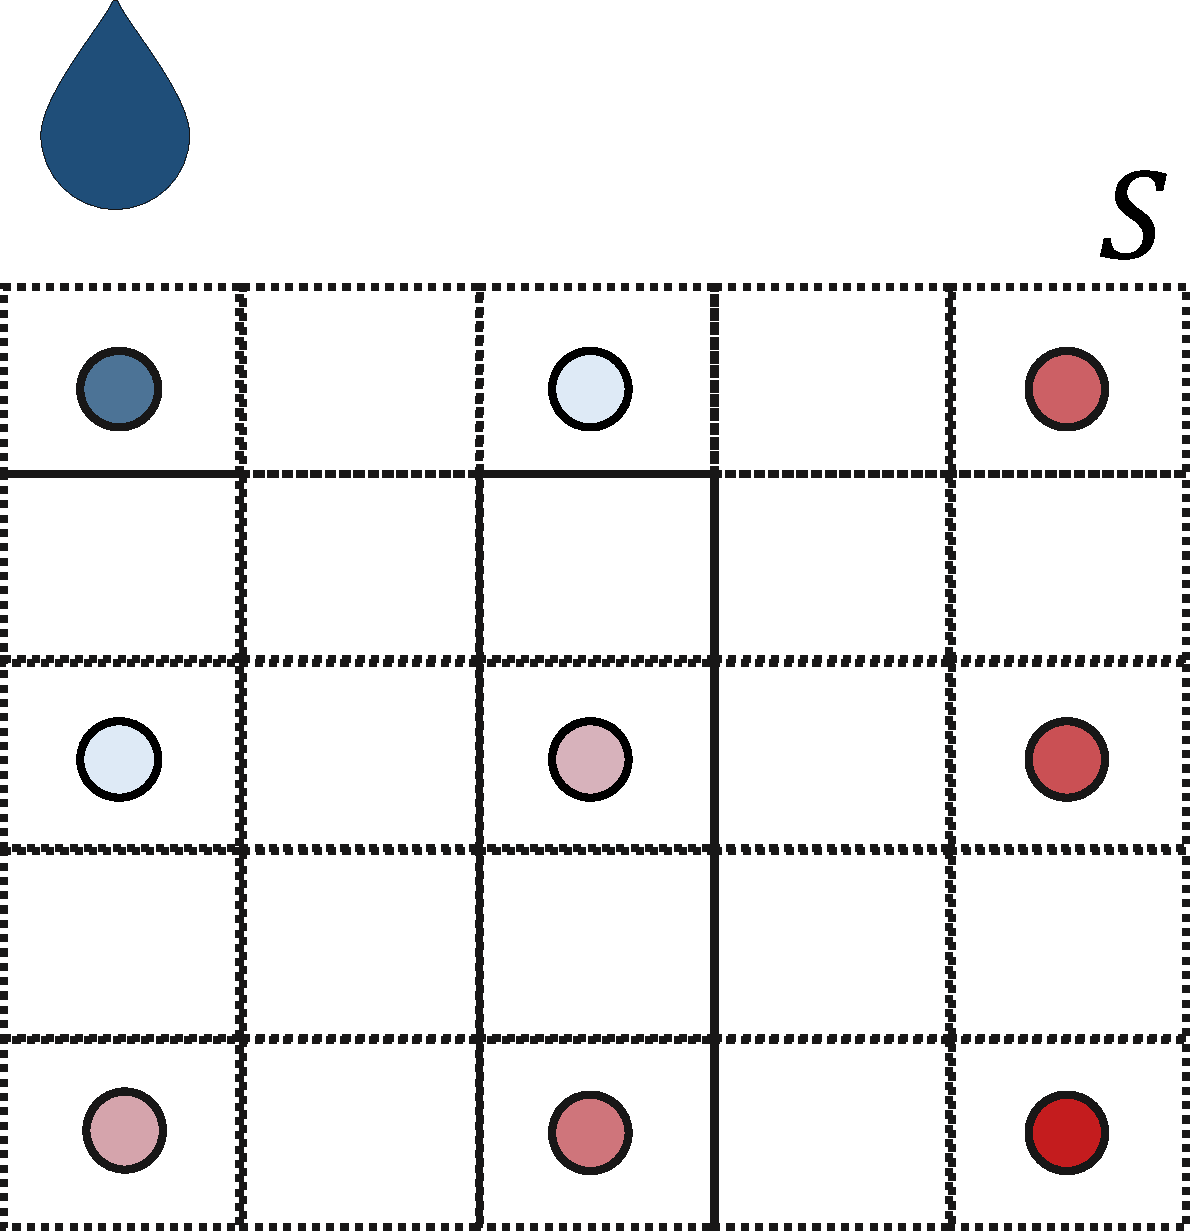
\includegraphics[scale=.15]{chapters/physics-aware/orchard/img/soil-moisture-sample.pdf}
\caption{Raw sensor grid}
\label{orchard-fig:moisture-sens}
\end{subfigure}
~
\begin{subfigure}[t]{.3\textwidth}
\centering
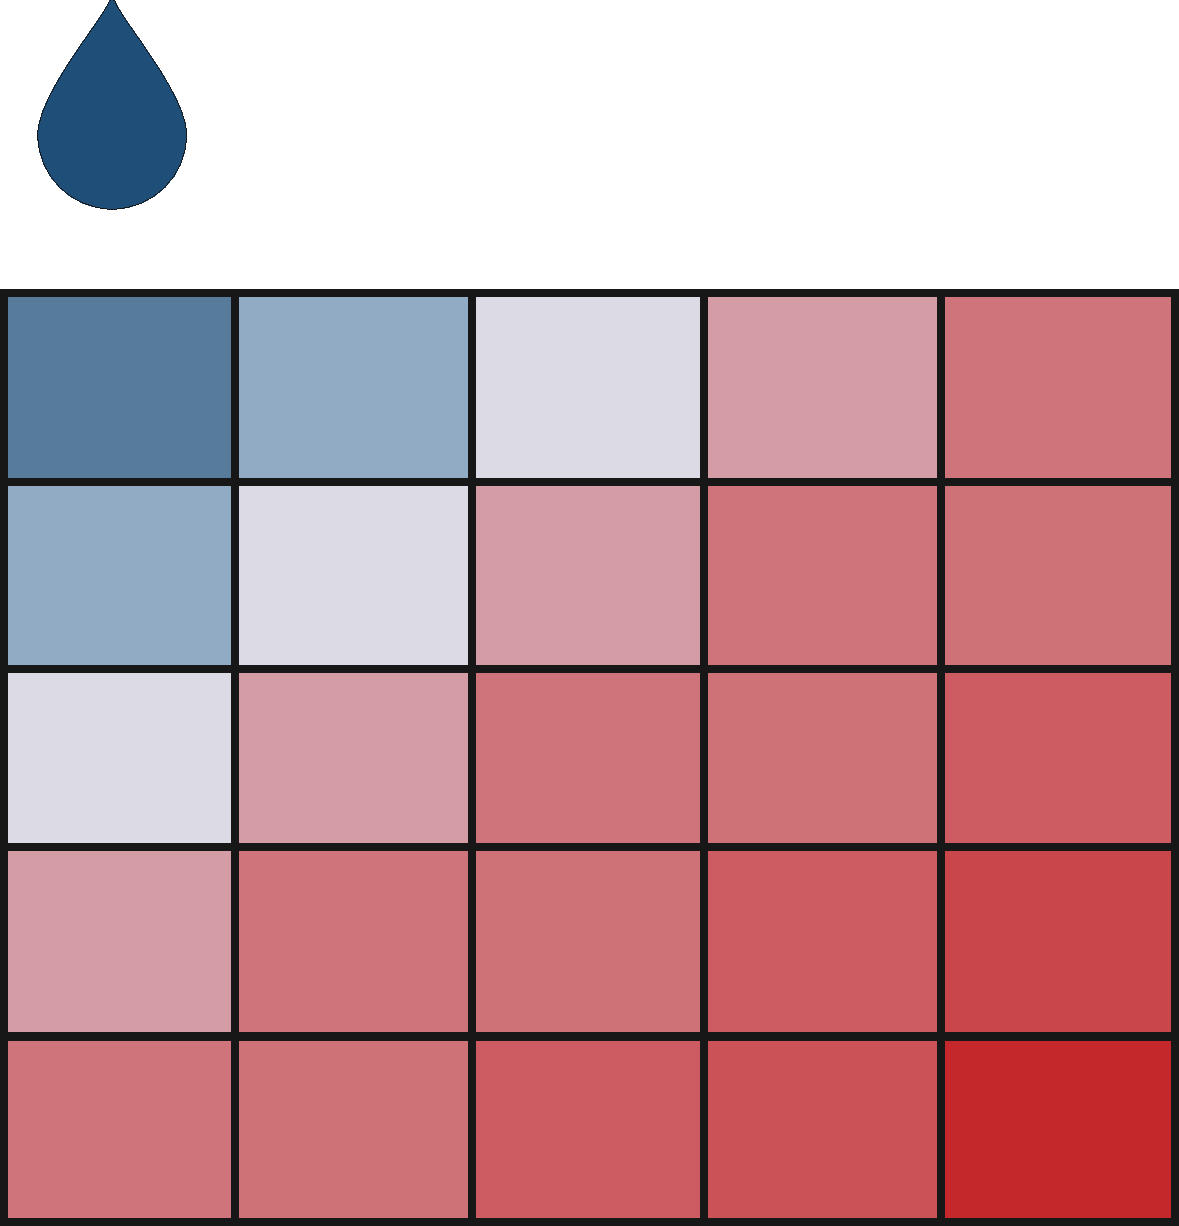
\includegraphics[scale=.15]{chapters/physics-aware/orchard/img/soil-moisture-profile.pdf}
\caption{Soil profile}
\label{orchard-fig:moisture-profile}
\end{subfigure}
\caption{Snapshot of soil moisture in a soil slice; the water drop represents a dripper.}
\label{orchard-fig:moisture}
\end{figure}

The assimilation process maps in-situ sensor data to a state of the crop model.
This is used as the initial state of the crop model, in this way the forecast begins from an actual soil condition (\Cref{orchard-fig:moisture-cont}).
Of course, the more sensors (e.g., gypsum-blocks; \Cref{orchard-fig:moisture-sens}), the better the granularity of the sampling and the accuracy of the initial state.
As in \Cref{physics-aware-chap:pluto}, such accuracy also depends on the sensor layout: the higher the dimensionality of the layout, the fewer the assumptions to be made:
\begin{itemize}
    \item most of the approaches in the literature rely on a single sensor and assume the soil moisture to be constant over the whole soil volume;
    \item a one-dimensional (1D) grid relies on a column/row of sensors and assumes the soil moisture to be constant over horizontal/vertical planes;
    \item a two-dimensional (2D; \Cref{orchard-fig:moisture-sens}) grid relies on a 2D matrix of sensors and assumes the soil moisture to be constant over adjacent slices;
    \item a three-dimensional (3D) grid measures soil moisture as is and makes no symmetry assumptions.
\end{itemize}

Due to the size, energy requirement, and cost of sensors, it is not feasible to adopt sensor grids as fine-grained as the ones simulated by the model; in other words the number of simulated cells ($|SM|$) is sensibly greater than the number of in-situ sensors.
In
% \cite{DBLP:journals/cea/FranciaGG22}
\Cref{physics-aware-chap:pluto}, we provide several \textit{profiling functions} that approximate the soil moisture sampled by a coarse-grained 2D/3D sensor grid to a \textit{refined grid} with finer granularity (\Cref{orchard-fig:moisture-profile}).
Orchard3D-Lab is pluggable and supports both feature-aware and feature-unaware profile functions.

% For the sake of conciseness, we describe the linear profiling function in a 2D scenario.
% Given a 2D sensor grid, the profiling function carries out a bi-linear interpolation of soil moisture.
% The approach consists of two phases (\Cref{orchard-fig:statistical-profiling-function-explanation}).
% For each point to be calculated: (i) we find the four sensors that determine the minimum bounding rectangle enclosing it (\Cref{orchard-fig:statistical-profiling-function}); then (ii) we interpolate along the first axis obtaining the moisture values on intermediate points and we determine the desired value by interpolating the intermediate values along the second axis (\Cref{orchard-fig:bilinear-interpolation}).

% \begin{figure}[t]
% \centering
% \begin{subfigure}[t]{.45\textwidth}
% \centering
% 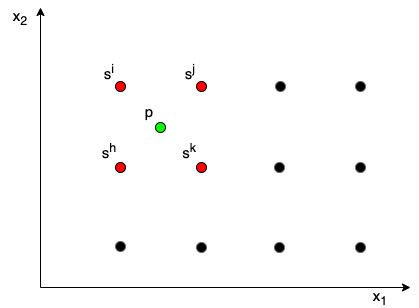
\includegraphics[scale=.4]{chapters/physics-aware/orchard/img/statistical_profiling_function.png}
% \caption{Bounding rectangle: in green the point to be approximated, in red the sensors enclosing it.}
% \label{orchard-fig:statistical-profiling-function}
% \end{subfigure}
% ~
% \begin{subfigure}[t]{.45\textwidth}
% \centering
% 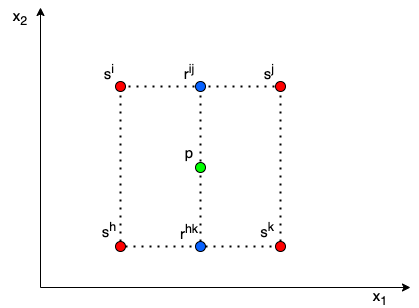
\includegraphics[scale=.4]{chapters/physics-aware/orchard/img/bilinear_interpolation.png}
% \caption{Bilinear interpolation: blue values $r$s are interpolated first, then $p$.}
% \label{orchard-fig:bilinear-interpolation}
% \end{subfigure}
% \caption{A 2D example of the profiling function.}
% \label{orchard-fig:statistical-profiling-function-explanation}
% \end{figure}

To ensure a precise sensing we consider 2D and 3D sensor grids since they rely on fewer symmetry assumptions.
Symmetry assumptions also depends on the dripper layout.
In this work, we refer to single-line dripper watering system (\Cref{orchard-fig:simmetries})
where the sensor grid is orthogonal to the dripper line (\Cref{orchard-fig:moisture-sens}). 
% The profiling function is applied to sensor data to obtain a refined grid (\Cref{orchard-fig:moisture-profile}), the $DataAssimilation$ function is implemented as follows.
The $DataAssimilation$ function relies on the profiling function to obtain a refined grid from a sensor grid (\Cref{orchard-fig:moisture-profile}), then it applies the necessary geometric transformations to complete the whole soil volume (i.e., the simulator state):
\begin{itemize}
    \item given a 2D refined grid, $SM$ is obtained by translating the refined grid along $y$ axis and by reflection on the $x$ axis (\Cref{orchard-fig:simmetries});
    \item given a 3D refined grid, $SM$ is obtained by reflection one the $x$ and $y$ axes.
\end{itemize}

 \begin{figure}[t]
	\centering
	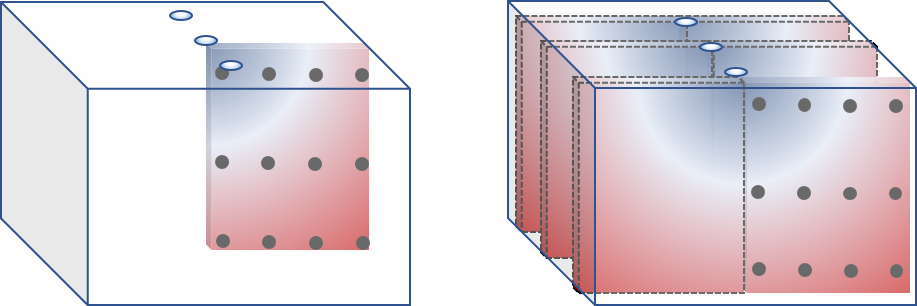
\includegraphics[scale=0.7]{chapters/physics-aware/orchard/img/Simmetries.png}
	\caption{Transforming a 2D sensor grid (left) into a state of the crop model (right) through translation and reflection geometric transformations.}
	\label{orchard-fig:simmetries}
\end{figure}


\subsection{Parameter Tuner}

Due to the huge number of parameters (\Cref{tab:parameter}), manual or brute-force tuning of the crop model is unfeasible.
% The Parameter Tuner lightens the user in the overwhelming practice of finding a promising configuration of parameters.
In the literature, there are numerous optimization methods that aim at finding the best configuration over huge search spaces \cite{luo2017automating}.
All of them are constrained under an exploration budget in terms of execution time or configurations to visit.
First they evaluate the performance of an initial (possibly random) configuration, then they converge to better configurations by smartly exploring a fraction of the search space.
We leverage an approach based on bayesian optimization \cite{frazier2018tutorial} which learns a model of the search space to explore the most promising regions; while the configurations are explored, bayesian optimization updates its model until the exploration budget elapses and the best-explored configuration is returned.
The chosen approach is based on the Blended-search \cite{wang2021flaml}, from the FLAML package, which enhances a common bayesian optimization model with the strengths of local search, and minimizes on the fly the total cost spent in finding bad configurations.

\begin{algorithm}[t]
\caption{Parameter Tuner}
\footnotesize
\begin{algorithmic}[1]
% \Require{$e$: Grounded extension of the Problem Graph}  
\Require{\Wt: weather time series, \It: irrigation time series, $X_{fix}$: fixed parameters, $X_{tun}$: tunable parameters, $budget$: maximum iterations, $\overrightarrow{S}$: sensor soil-moisture time series} 
\Ensure{$X_{tun}^*$: best parameter configuration}
    \State $SM_{Ass} \gets \textup{DataAssimilation}(\overrightarrow{S}_{0})$ \Comment{Assimilate the initial state}
    \State $H \gets \varnothing$ \Comment{History of explored configurations}
    \State $iteration \gets 0$ \Comment{Current iterations}
    \While{$iteration < budget$} \Comment{While some budget remains}
        \State $iteration \gets iteration + 1$ \Comment{... increase the iterations}
        \State $X'_{tun} \gets BayesianOpt(H)$ \Comment{... optimize the ``free'' parameters}
        \State \SMt $\gets \textup{CropModel}(SM_{Ass}$, \Wt, \It, $X'_{tun} \cup X_{fix})$ \Comment{... run the simulator}
        \State $e \gets error($\SMt, $\overrightarrow{S})$ \Comment{... get the error}
        \State $H \gets H \cup \{(X'_{tun}, e)\}$ \Comment{... add the configuration to the history}
    \EndWhile
    \State \Return $argmin_{X^*_{tun}~s.t.~(X^*_{tun}, e) \in H}{(e)}$ \Comment{Return the best configuration}
\end{algorithmic}
\label{alg:bayesian-optimization}
\end{algorithm}


The parameter tuner is detailed in \Cref{alg:bayesian-optimization} and takes as inputs: weather and irrigation time series, the soil moisture time series sampled by sensors (our ground truth), a maximum iteration budget, and the subsets of (manually) fixed and automatically-tunable parameters 
($X_{fix} \cup X_{tun} = X$ and, $X_{fix} \cap X_{tun} = \varnothing$, with $X$ being the parameters from \Cref{tab:parameter}).
The algorithm returns as output the configuration of parameters that allow \olab{} to produce the best approximation of real sensor values (i.e., of our ground truth).
Given the simulation states \SMt{} and the sampled soil moisture $\overrightarrow{S}$, the error of approximating $\overrightarrow{S}$ with \SMt{} is computed as follows
\begin{align}\label{orchard-eq:error}
error(\overrightarrow{SM}, \overrightarrow{S}) &= \frac{1}{|\overrightarrow{S}|} \sum_{\overrightarrow{S_t} \in \overrightarrow{S}} RMSE(\overrightarrow{SM_t}, \overrightarrow{S_t})\\
RMSE(\overrightarrow{SM_t}, \overrightarrow{S_t}) &= \sqrt{\frac{1}{|S_t|} \sum_{s_t \in S_t} (log(s_t) - log(sim_t)) ^ 2}
\end{align}

where $\overrightarrow{S_t}$ and  $\overrightarrow{SM_t}$ are the soil-moisture values at time $t$ from real sensors and from the simulator, respectively. Consistently, $s_t$ and $sim_t$ represent the soil moisture of a specific sensor/position. Finally, $error()$ averages the $RMSE()$ over all the samples in the time series. Soil moisture (i.e. $s_t$ and $sim_t$) ranges over several degrees of magnitude, thus the same nominal variation may have a different significance (e.g., a variation of $50cbar$ in the range of $[0, -100]~cbar$ has, by far, a higher impact  than in $[-100, -1000]~cbar$). By computing the logarithm we make variations comparable and in particular we make average meaningful.

The algorithm assimilates the initial state of the simulator from the first snapshot of the sampled soil moisture (Line 1) and initializes the history of explored configurations (initially empty; Line 2) and the number of iterations (Line 3).
While the iteration budget is not exhausted (Line 4), 
we increase the iterations (Line 5),
optimize the tunable parameters through bayesian optimization (Line 6),
forecast the soil moisture trend with the crop model (Line 7),
compute the approximation error (Line 8),
and add the explored configuration along with its error to the history (Line 9).
Finally, when the budget is exhausted, the best configuration is returned (Line 10). We recall that $BayesianOpt()$ carries out a smart exploration of the parameter search space that finds out good configuration even with a limited budget.

To the best of our knowledge, \olab{} is the only dramework that leverages this innovative family of optimization methods.
Other tools (e.g., HYDRUS) employed either local (e.g., the Marquardt-Levenberg algorithm) or model-free (e.g., genetic algorithms) optimization methods. 

\section{Empirical Evaluation}
The system has been tested on a kiwi orchard in the hills of central-northern Italy, part of a commercial farm that was selected to represent the real conditions for kiwi production in the area.
The tests refer to the period June-August 2022 for which weather, irrigation, and real soil moisture (our ground truth) time series were collected.
We verify how accurately the system, properly tuned, can simulate the real soil behavior.
Specifically, \Cref{orchard-ssec:settings} introduces the general experimental settings, \Cref{orchard-ssec:eval_end_to_end} evaluates the efficieny and effectiveness of our end-to-end approach, and finally \Cref{orchard-ssec:eval_tuner} provides the performance of the parameter tuner.

The implementation can be found on GitHub \footnote{\url{https://github.com/big-unibo/orchard3d-lab}} and a demo of our \olab{} visualization system is available on our website \footnote{\url{https://big.csr.unibo.it/projects/orchard3d-lab}}.

\begin{table}[H]
	\centering
	\scriptsize
	\begin{tabular}{p{1.2cm}p{5cm}p{7.5cm}}
 		\textbf{Type} & \textbf{Parameter} & \textbf{Value} \\
		\hline%\midrule
		Field & Location &  latitude = 44.28, longitude = 11.92, altitude = $62~m$\\
		& Slopes & horizontal = $-0.01~m \cdot m^{-1}$, vertical = $-0.025~m \cdot 
 m^{-1}$ \\
		& Mound & slope = $0.2~m \cdot m^{-1}$, width = $1~m$ \\
		& Water table & None\\ 
		\hline%\midrule
	    \multirow{2}{1cm}{Soil Layer*}	& Thickness & $0.9~m$ \\
		& Texture & sand = 30 \%, silt = 30 \%, clay = 40 \% \\ % esiste mappa dei suoli in regione
		& \textbf{Ksat} & $1.1 \cdot 10^{-6}$  \\ % valore di default da soil editor (fitting non lineare, oppure fitting lineare con un ordine +/- rispetto a valore di default). Da convertire da cm/gg a m/s
		& $\pmb{\theta_s}$ & 0.5 $m^3 \cdot m^{-3}$\\  
		& $\pmb{\theta_r}$ & 0.03 $m^3 \cdot m^{-3}$\\  
		& $\pmb{\alpha}$ & 1.9 $m^{-1}$\\  
		& $\mathbf{n}$ & 1.5 \\
		& \textbf{he} & 0.23 $m H_2O$ \\ 
		& b & None \\ 
		\hline%\midrule
		Plant* & Position & first = (0.0, -0.3)\\
		& \textbf{Radius} & 1.6 $m$\\
		& \textbf{Leaf area index} & 4.5 \\ % se distribuzione delle piante uniforme (i.e., molto vicine), possiamo tenerlo fisso
		& \textbf{Root depth} & 0.8 $m$ \\
		& \textbf{Root deformations} & $root_x = 0.0$, $root_z = 0.8$ \\ 
		& \textbf{Kc max} &  2.6\\
		& \textbf{fRAW} & 0.5\\
		\hline%\midrule
        \multirow{2}{1cm}{Irrigation elem*} & Type & Single-line Dripper \\
		& Position & first = (0.0, -0.67), second = (0.0, 0.0), third = (0.0, 0.67)\\
		\hline%\midrule		
		Model & Geometry &  length = $2~m$, width = $2~m$ , depth = $0.8~m$ \\
		& Cell size  &  min = $0.01~m$, max = $0.04~m$  \\
% 		& Boundary conditions $\in [free\_drainage, default]$ & \textcolor{orange}{Description needed}\\ 
		& Retention curve & mod. Van Genuchten\\ 
	    & Conductivity mean &  log \\
		& Conductivity H/V Ratio  &  1.0 \\
		\bottomrule
	\end{tabular}%
	\begin{tablenotes}
      \scriptsize
      \item Types with * can have several elements. Parameters in bold are targeted by the parameter tuning.
    \end{tablenotes}
        \caption{System parameters values for our case study.}

	\label{tab:parameter_instances}%
\end{table}%

\subsection{General Experimental Setup}
\label{orchard-ssec:settings}

The total length of the field is $170~m$, the inter-row distance (plant to plant) is $4.5~m$, while the intra-row distance is $2~m$.
The implant is located in Errano (Faenza, Emilia-Romagna, Italy), having a latitude of 44.28, a longitude of 11.92, and an altitude of $62~m$.
The slopes were set based on field measurements performed with a total station, specifically: -1 $m \cdot m^{-1}$ horizontally and 2.5 $m \cdot m^{-1}$ vertically.
From the center of the intra-row, a $1~m$ long mound with 20 $m \cdot m^{-1}$ of slope extends in both directions.
No water table was observed.

\subsubsection{System Parameters}

\Cref{tab:parameter_instances} reports the system parameters for the simulated portion.

\begin{figure}[t]
    \centering
    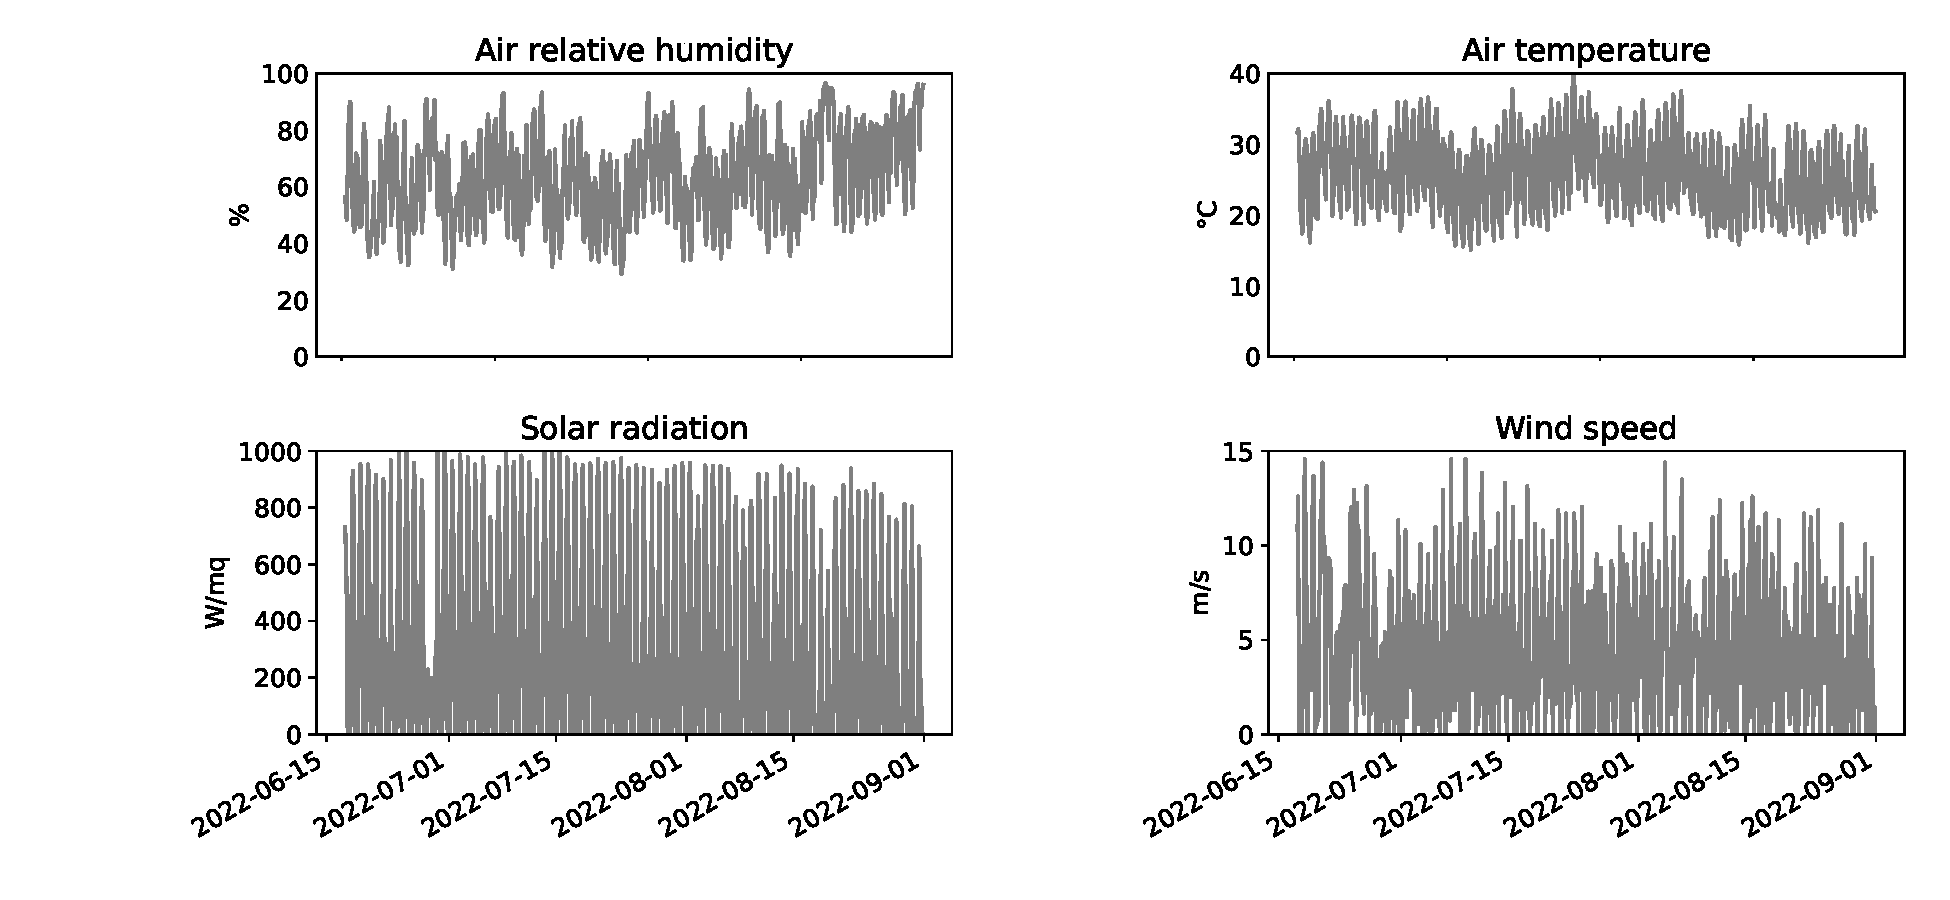
\includegraphics[scale=.45]{chapters/physics-aware/orchard/img/meteo.pdf}
    \caption{Weather time series throughout the simulation period.}
    \label{orchard-fig:meteo}
\end{figure}

Basic soil properties were measured at the site, a single layer of $0.9~m$ with a loamy texture (30 \% sand, 30 \% silt, and 40 \% clay) based on the International Soil Science Society (ISSS) classification system.
Soil water retention parameters were obtained from the parameter tuning procedure (a saturation threshold of $0.5~L^3 \cdot L^{-3}$, a residual of $0.03~L^3 \cdot L^{-3}$, and the related Van Genuchten parameters).

According to the implant layout, for the simulated plant we considered three drippers in a single line ($0.66~m$ apart from each other).
The root system has been estimated to have a radius of $1.6~m$ and a depth of $0.8~m$. According to \Cref{orchard-sec:root} roots are taproot shaped; the $root_x$ and $root_z$ determine the shape shown in \Cref{orchard-fig:root}. The volume of the simulated parallelepiped is $2~m\cdot2~m\cdot0.8~m$ (the product of length, width, and depth).
This allows to properly simulate the whole root system.
The domain is discretized with a dynamic cell size: both length and width are set to $0.125~m$, the depth ranges from $0.01~m$ to $0.04~m$.
Specifically, a geometrical progression was chosen in the first $0.2~m$ of soil.


\subsubsection{Weather, Watering, and Soil Moisture Time Series}
\label{orchard-sec:time_series}

\begin{figure}[t]
    \centering
    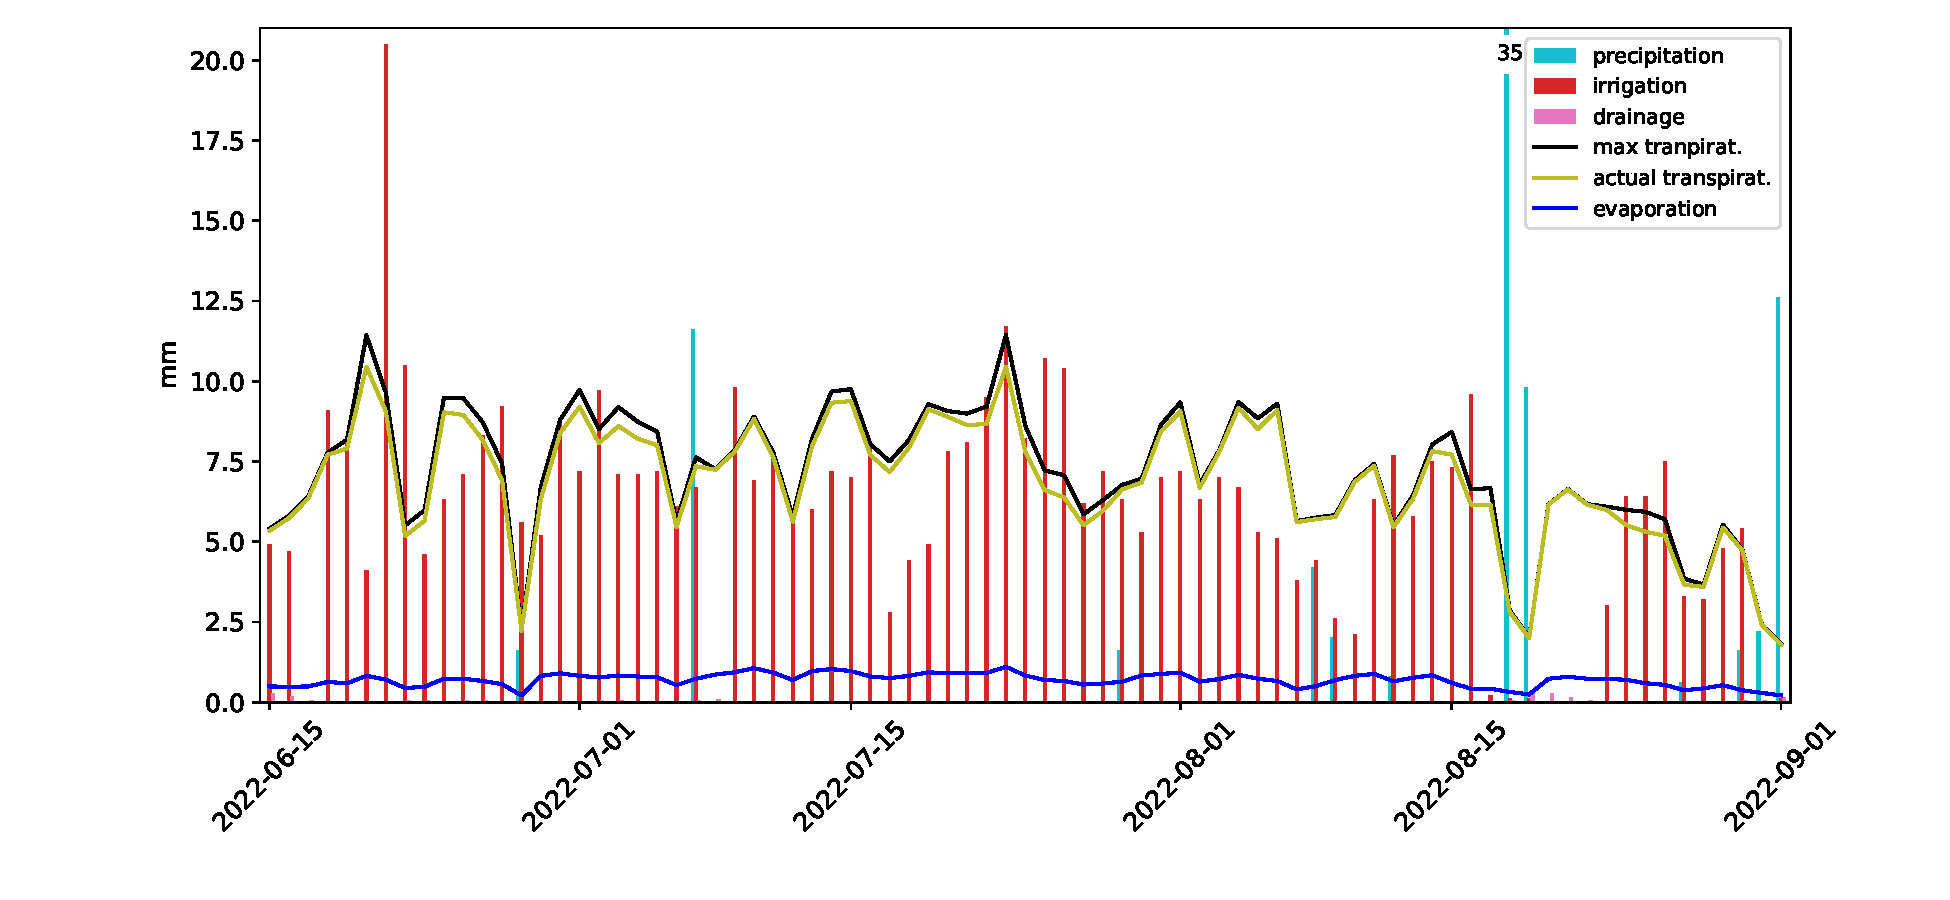
\includegraphics[scale=.45]{chapters/physics-aware/orchard/img/water_balance.pdf}
    \caption{Water balance throughout the period.}
    \label{orchard-fig:water_balance}
\end{figure}

All data were sampled hourly.
Weather and watering variables, to be provided as inputs to the model, were  collected at the site through a weather station and a water meter, respectively.
We monitored the field from May to October 2022, and selected the period of the actual irrigation season: from June 21th to August 31th.
\Cref{orchard-fig:meteo} depicts the trend of air humidity, air temperature, solar radiation, and wind speed through the whole period.
In general, air humidity and temperature show a hot and damp summer, with a peak of 39°C of air temperature and 97.7 \% of humidity.
The period was poorly ventilated, and solar radiation is typical of the area with values ranging from about 350  in March to 750 W m$^{-2}$ in July.
The water balance in \Cref{orchard-fig:water_balance} provides a detailed description of the water dynamics of the orchard.
%
We observed an extremely dry season w.r.t. precipitation; the only significant rain was detected around mid August.
%
Hence, the drainage is present only after the rains of August and a constant amount of irrigation was mandatory in the remainder extent of time.
%
The evaporation is always contained, below or around 1 mm/d (which corresponds to one liter per square metre) due to the kiwi leaf cover which shades the ground.
%
On the other hand, the transpiration demand is very high, some days even over 10 mm/d, but irrigation amounts and schedule are adequate for the demand---apart from the excessive irrigation of 20 mm in June.
%
Therefore, the plant never experienced water stress, as can be seen from the fact that the actual transpiration  is always equal to or close to the maximum required by the weather conditions.

\begin{figure}[t]
    \centering
    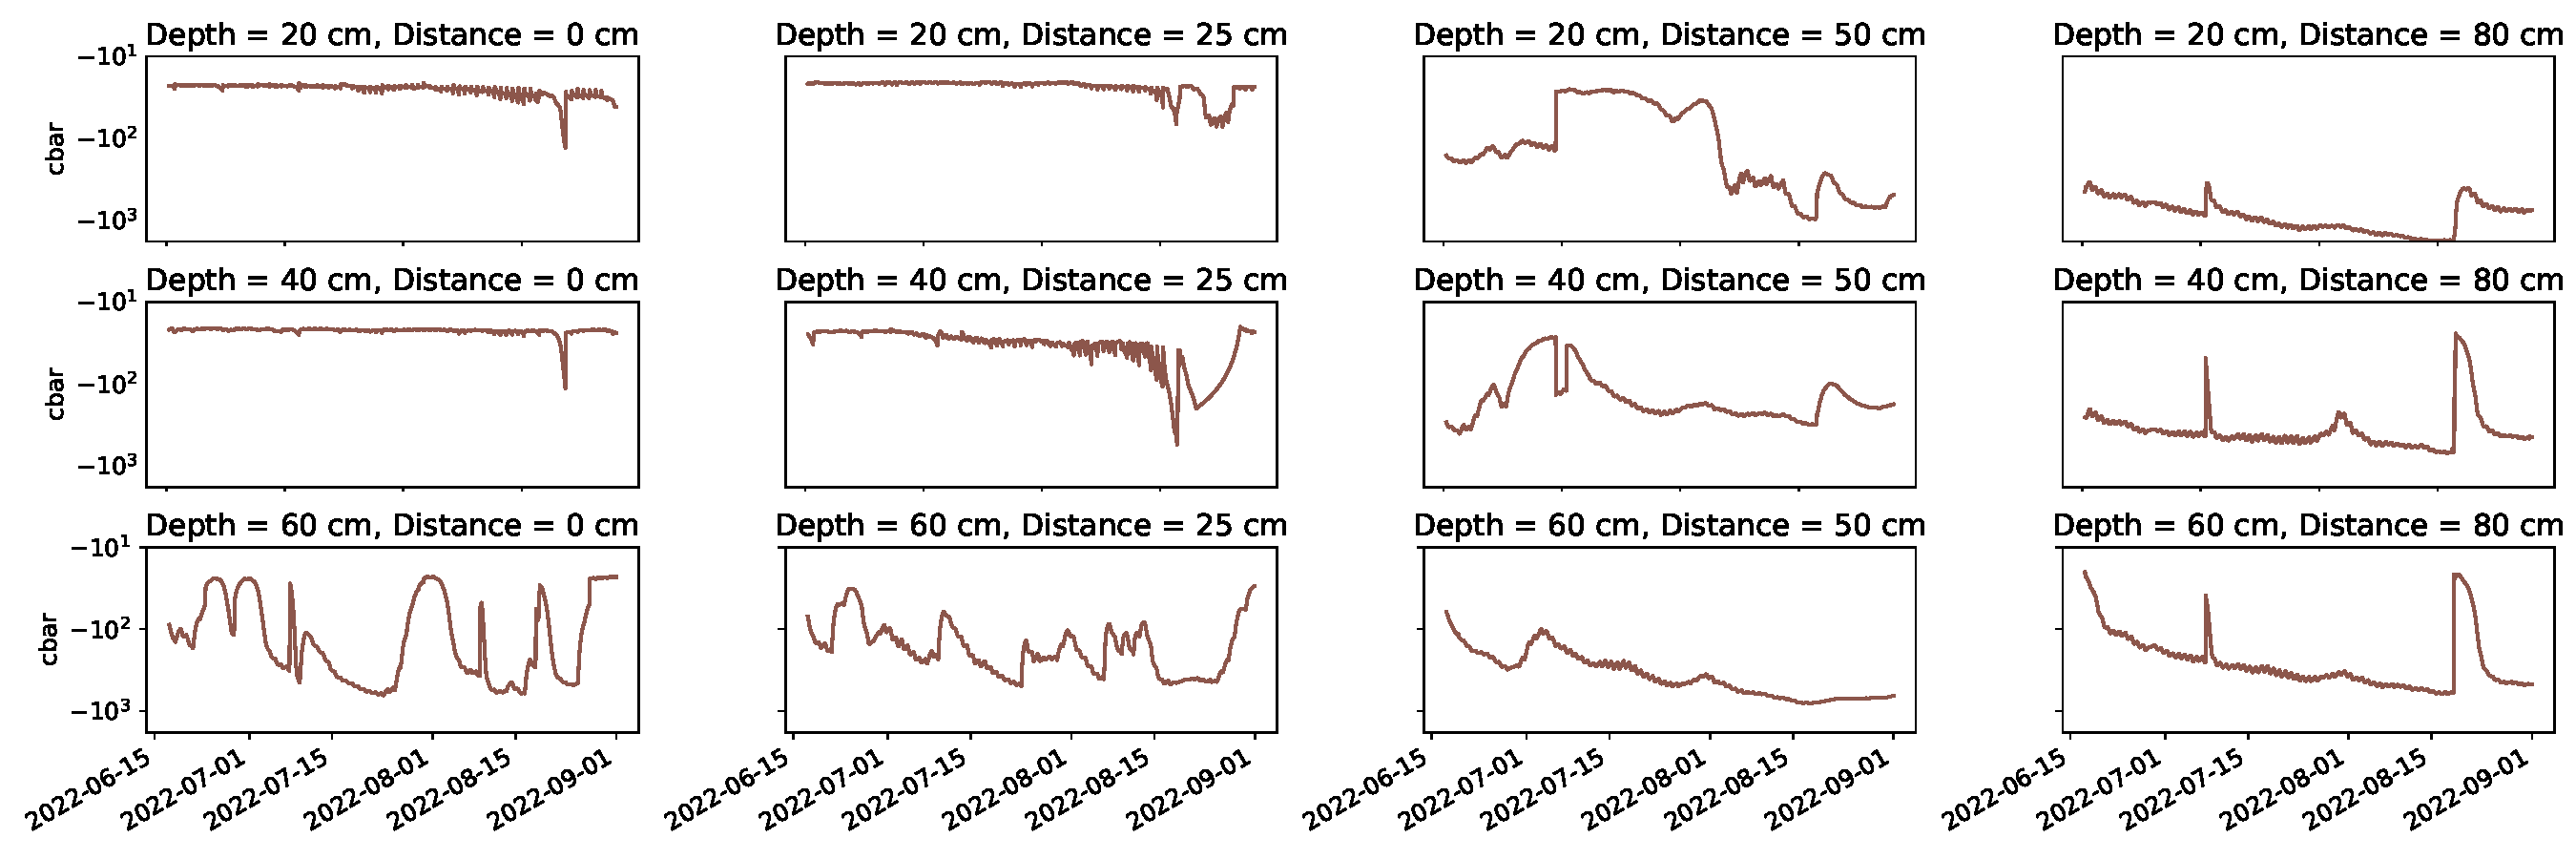
\includegraphics[scale=.3]{chapters/physics-aware/orchard/img/ground_potential.pdf}
    \caption{Ground potential time series of the 12 sensors throughout the simulation period. }
    \label{orchard-fig:ground_potential}
\end{figure}

As to the soil moisture, we employed a 2D sensor grid of 12 GB-1 Gypsum Sensor Blocks (Delmhorst Inc.). As shown in \Cref{orchard-fig:ground_potential}, sensors were organized on three different depths ($0.2~m, 0.4~m, 0.6~m$ on the $z$ axis), with four elements per level on the $x$ axis ($\approx 0.25~m$ to each other). The grid was hortogonal to the $y$ axis (i.e. the intra-row line), with $0.2~m$ of translation from the plant, with the top left corner under the dripper.


\subsection{End-to-end Approach Performance}
\label{orchard-ssec:eval_end_to_end}

In this section we provide a set of tests aimed at verifying the simulation effectiveness.
The system parameters tuning procedure is run over a two-weeks period (June 21th - July 5th), while the remaining samples (July 6th - August 31th) were exploited for testing.

We tested Orchard3D-Lab with three different forecasting horizons: 1, 3, and 7 days ahead.
For every timestamp $t$ in the testing period, we run the assimilation procedure (see \Cref{orchard-ssec:ass}) to compute the initial state $SM_{Ass}$ and then we fed Orchard3D-Lab providing with \Wt and \It  according to the forecasting horizon.
For instance, given an horizon of 3 days, Orchard3D-Lab: (i) assimilates the soil moisture of the first sample, (ii) iterates the simulation for the duration of 72 samples, (iii) calculates the error between observed and final simulated samplings.

\paragraph{Efficiency Tests} In terms of computation time, forecasting the soil moisture in a future state depends on the current water content of the soil and the amount of irrigation/precipitation of each hour (the more the watering, the more expensive the calculation).
Tests are run on an Intel Core i7 machine running at 3.20 GHz with 64 GB of main memory.
Throughout the whole period, we observed an average of 2 seconds in forecasting the soil moisture of the next hour.
Hence, a computation time of: 48 seconds for a 1-day horizon, 144 seconds ($\approx$ 2 minutes) for a 3-day horizon, and 336 seconds ($\approx$ 5 minutes) for a 7-day horizon.

\begin{figure}[t]
    \centering
    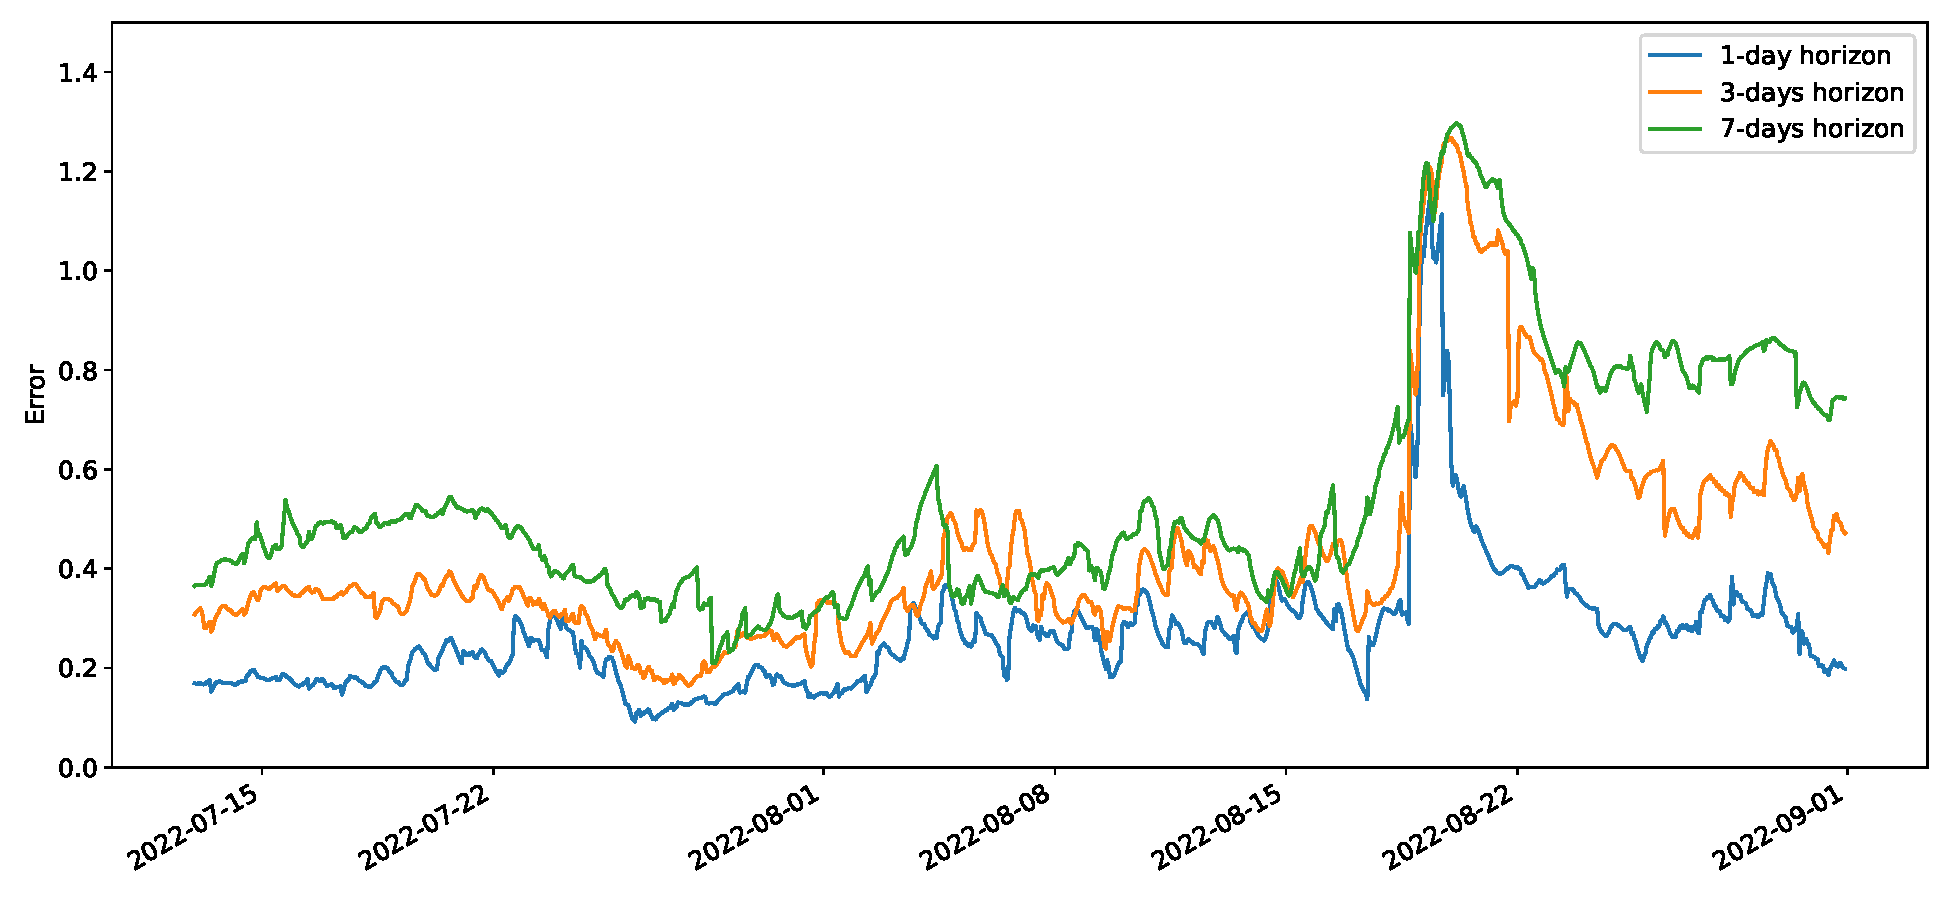
\includegraphics[scale=.4]{chapters/physics-aware/orchard/img/forecasting_avg_with_forbidden_sensors.pdf}
    \caption{Error of \Cref{orchard-eq:error} in forecasting 1, 3, and 7 days ahead throughout the period.}
    \label{orchard-fig:forecasting_avg}
\end{figure}

\paragraph{Effectiveness Tests} \Cref{orchard-fig:forecasting_avg} reports the \textit{error} metric in \Cref{orchard-eq:error} for the three different forecasting horizons.
\olab{} was able to achieve good performance in forecasting soil moisture during the whole season, with an exception occurred around mid-August.
Given the very dry season and the heavy rainfall in those days, the soil presented unexpected macropores and cracks is the sub-surface layers.
This resulted in a non-uniform distribution and unexpected changes in the soil moisture dynamics, which the model was unable to fully capture due to its limitation in accounting for preferential flows.
Yet, it is worth to notice how the assimilation mechanism allows \olab{} to recognize such events, reset to the actual state, and hence quickly reduce the error.
Forecasts with shorter horizons assimilate earlier and response faster to the change.

\begin{figure}[t]
    \centering
    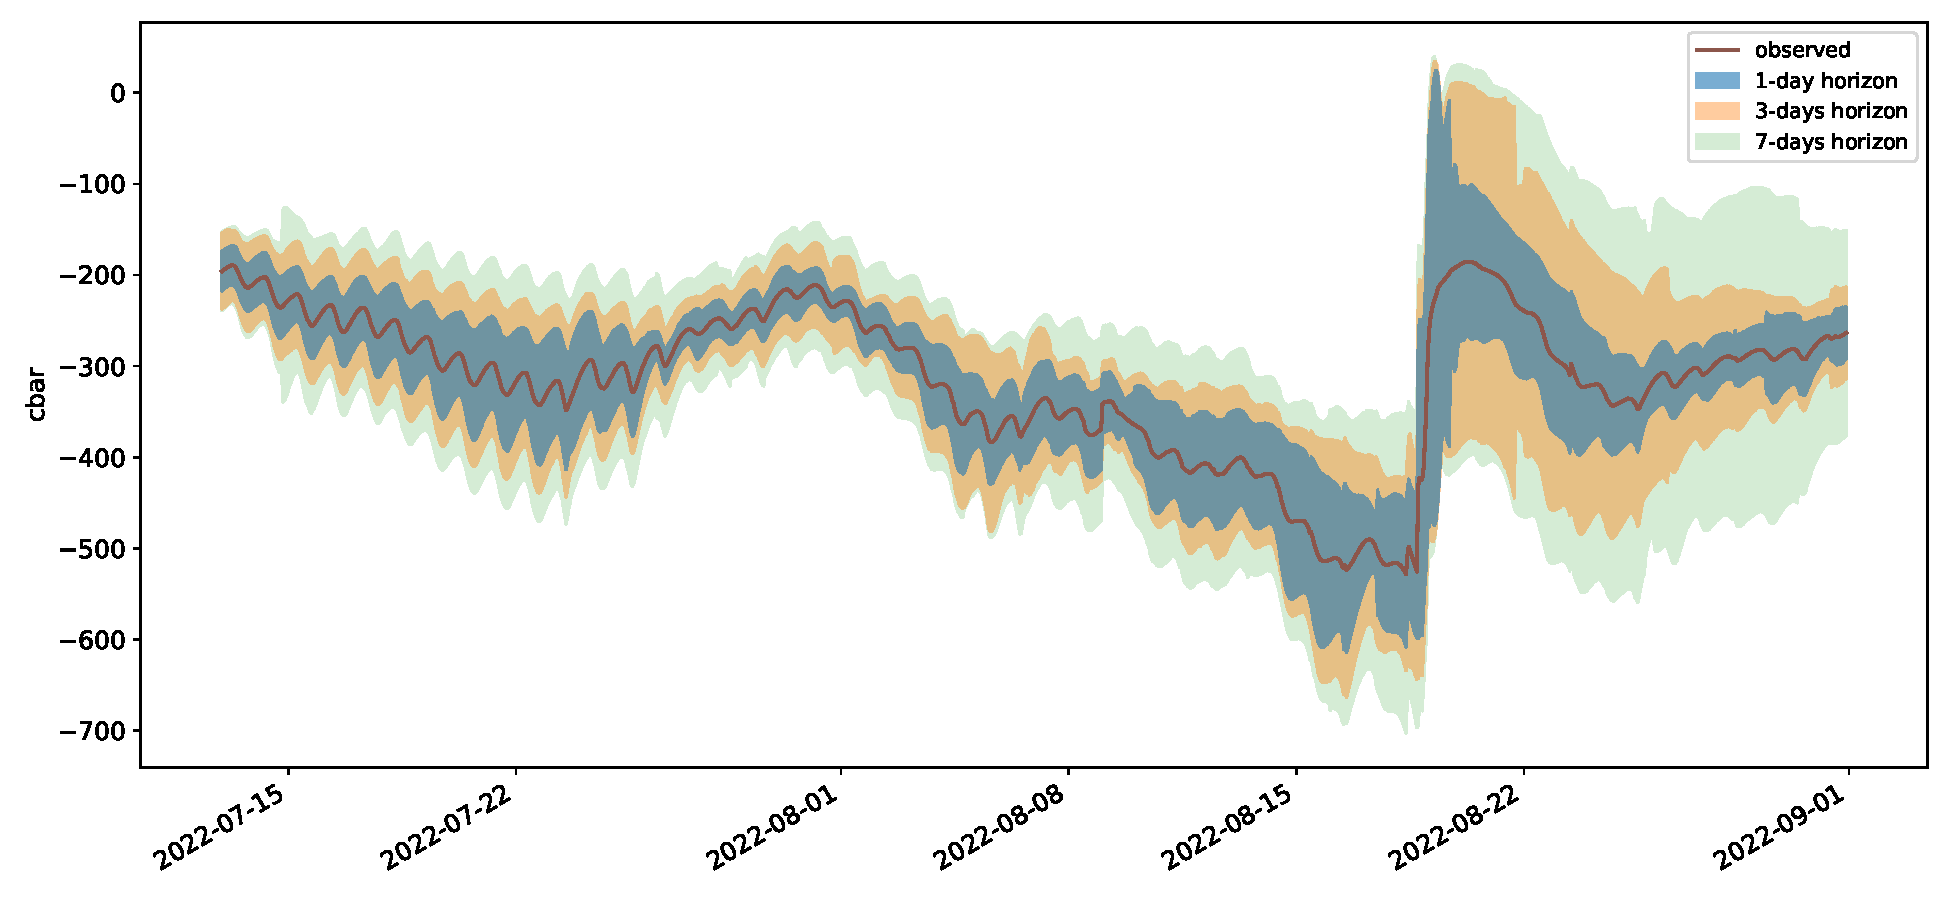
\includegraphics[scale=.4]{chapters/physics-aware/orchard/img/forecasting_std_with_forbidden_sensors.pdf}
    \caption{Averaged (observed) ground potential and confidential interval according to the error of \Cref{orchard-eq:error}.}
    \label{orchard-fig:forecasting_std}
\end{figure}

Overall, the average of the error is kept at: 0.27 for the 1-day horizon, 0.43 for the 3-days horizon, and 0.55 for the 7-days horizon.
%; which translates into a forecast that varies -- respectively -- 30\%, 50\%, and 70\% of observed ground potential.
Reasoning only on errors makes it difficult to understand if forecasts are accurate enough to support precision watering policies. For this reason in \Cref{orchard-fig:forecasting_std} we report the actual gap between observed and forecasted soil moisture.
More in details, the average soil moisture measured is reported as soil water potential (cbar) and the gap as range interval of forecasted values.

It is apparent, that forecasted water potential is closed enough to support watering policies formulation. Note that, as water potential is not linear, the ranges of values are smaller when the water potential is closer to the field capacity (i.e., the soil is more saturated). In other words, the same error in absolute terms has different impacts at different levels of soil saturation. \olab{} ensures the same relative error at different saturation levels, and this results in wider ranges of values when the soil is less saturated.

\begin{figure}[t]
    \begin{subfigure}[b]{0.47\textwidth}
        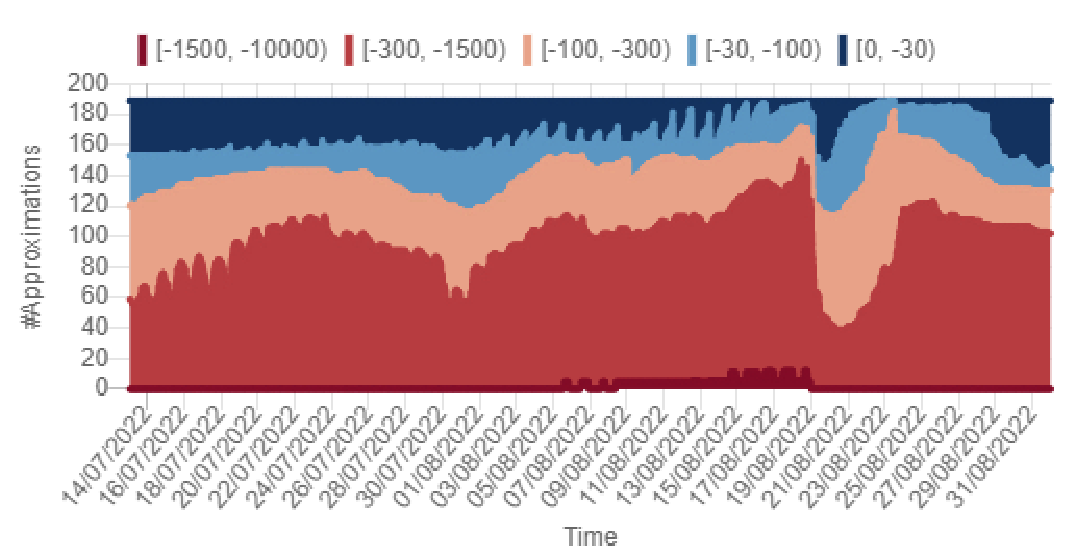
\includegraphics[width=\textwidth]{chapters/physics-aware/orchard/img/obs_stacked.pdf}
        \caption{observed}
        \label{orchard-fig:stacked_a}
    \end{subfigure}
    \hfill
    \begin{subfigure}[b]{0.47\textwidth}
        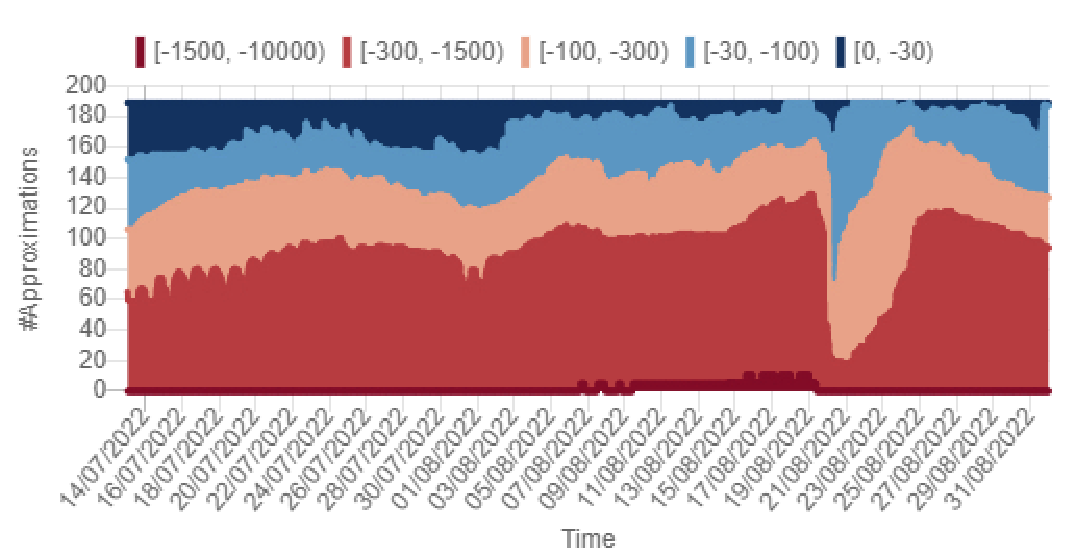
\includegraphics[width=\textwidth]{chapters/physics-aware/orchard/img/1gg_stacked.pdf}
        \caption{1-day horizon}
        \label{orchard-fig:stacked_b}
    \end{subfigure}
    \\
    \begin{subfigure}[b]{0.47\textwidth}
        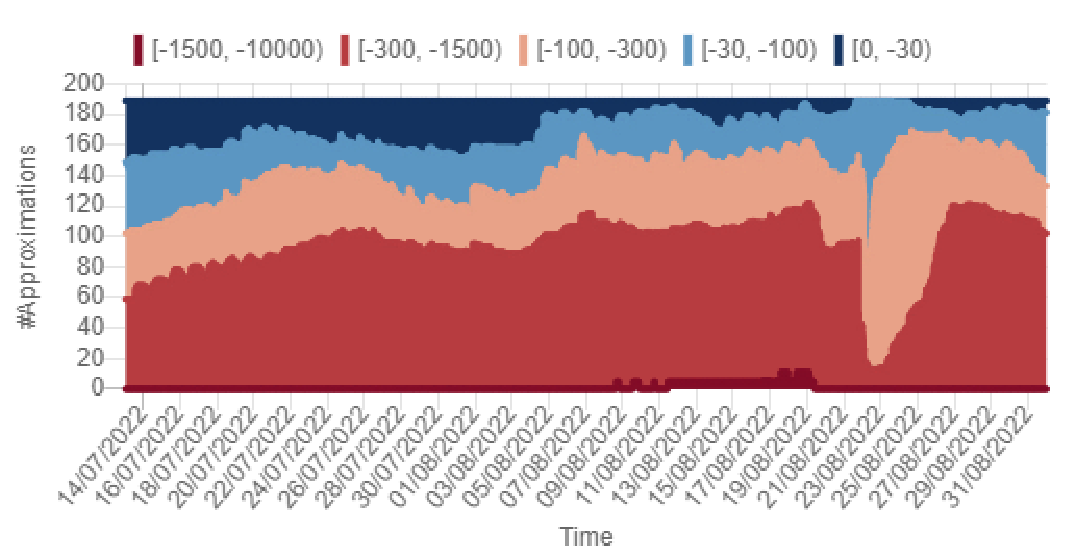
\includegraphics[width=\textwidth]{chapters/physics-aware/orchard/img/3gg_stacked.pdf}
        \caption{3-days horizon}
        \label{orchard-fig:stacked_c}
    \end{subfigure}
    \hfill
    \begin{subfigure}[b]{0.47\textwidth}
        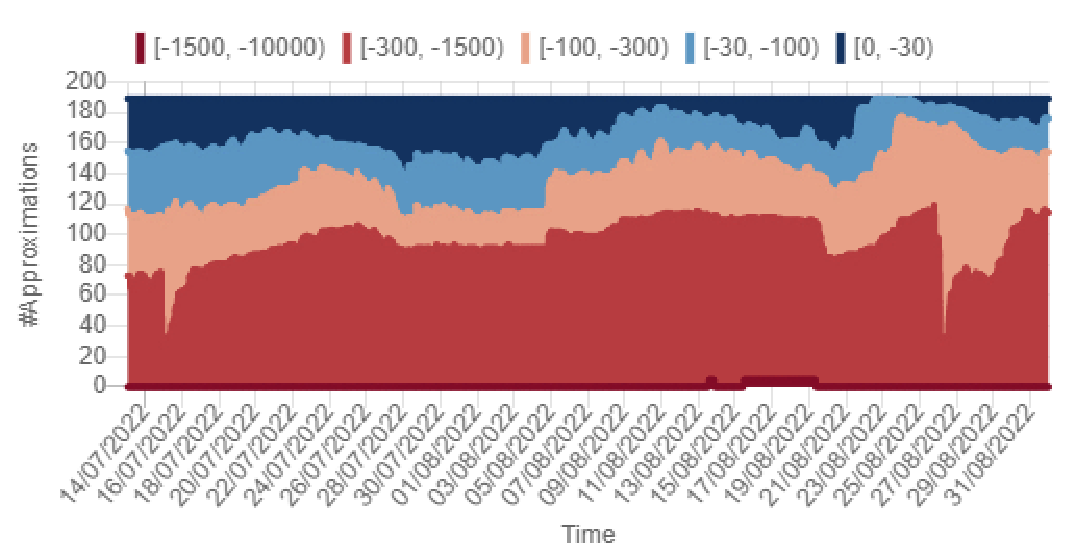
\includegraphics[width=\textwidth]{chapters/physics-aware/orchard/img/7gg_stacked.pdf}
        \caption{7-days horizon}
        \label{orchard-fig:stacked_d}
    \end{subfigure}
    \caption{Soil moisture trend over the period.}
    \label{orchard-fig:stacked}
\end{figure}

\begin{figure}[t]
    \begin{subfigure}[b]{0.47\textwidth}
        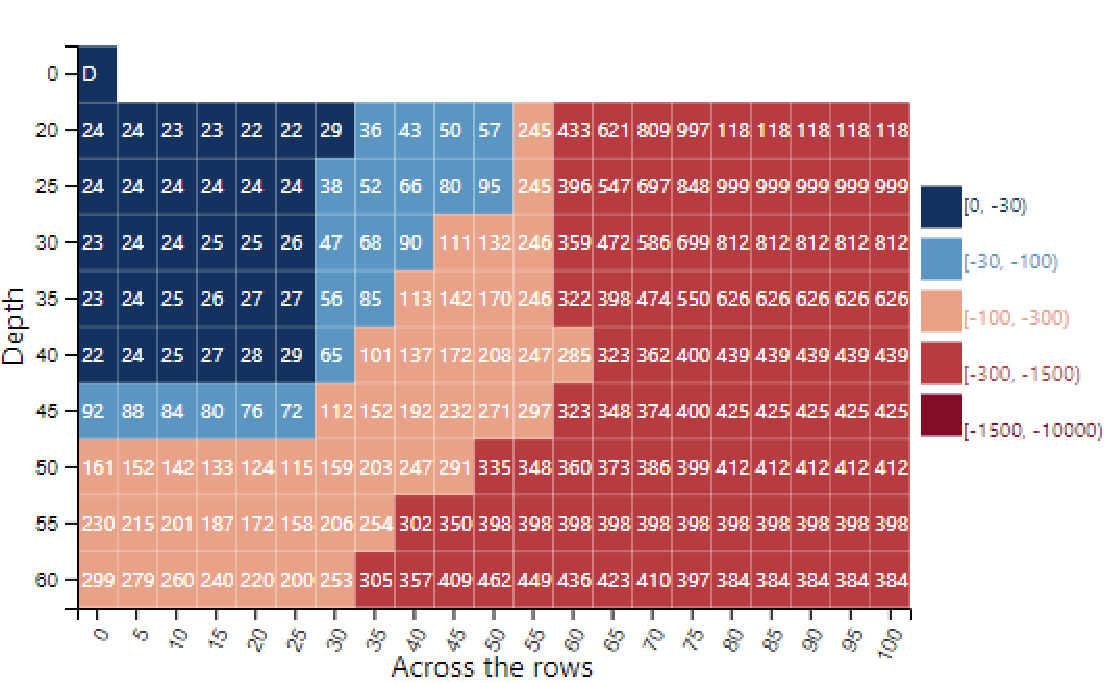
\includegraphics[width=\textwidth]{chapters/physics-aware/orchard/img/obs_profile.pdf}
        \caption{observed}
        \label{orchard-fig:profile_a}
    \end{subfigure}
    \hfill
    \begin{subfigure}[b]{0.47\textwidth}
        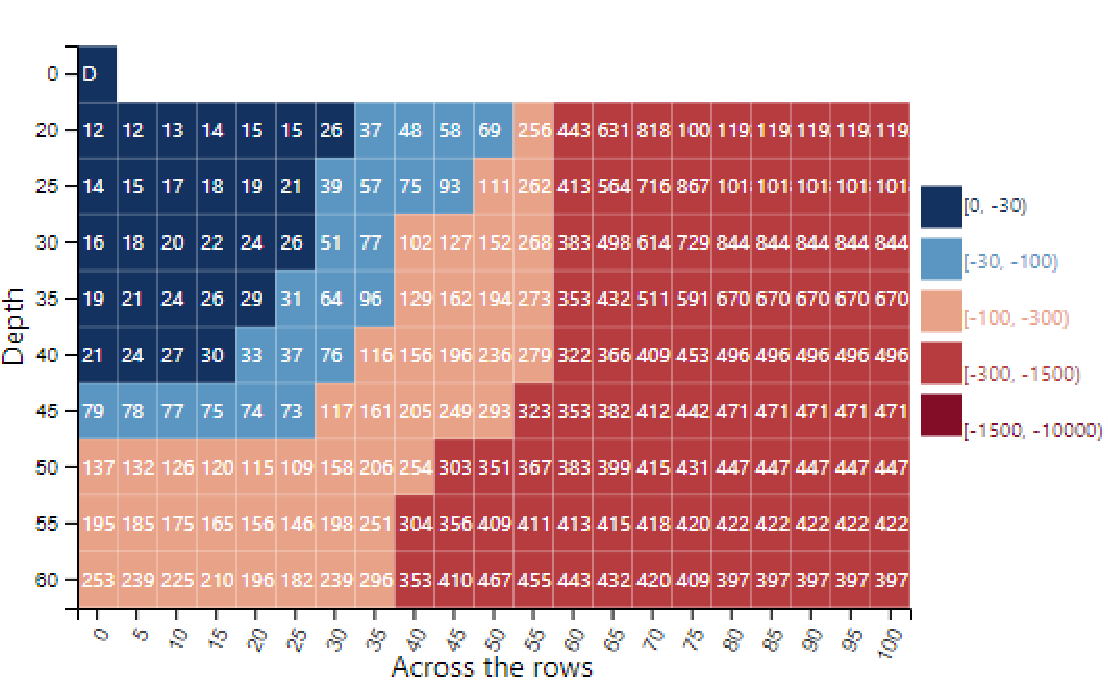
\includegraphics[width=\textwidth]{chapters/physics-aware/orchard/img/1gg_profile.pdf}
        \caption{1-day horizon}
        \label{orchard-fig:profile_b}
    \end{subfigure}
    \\
    \begin{subfigure}[b]{0.47\textwidth}
        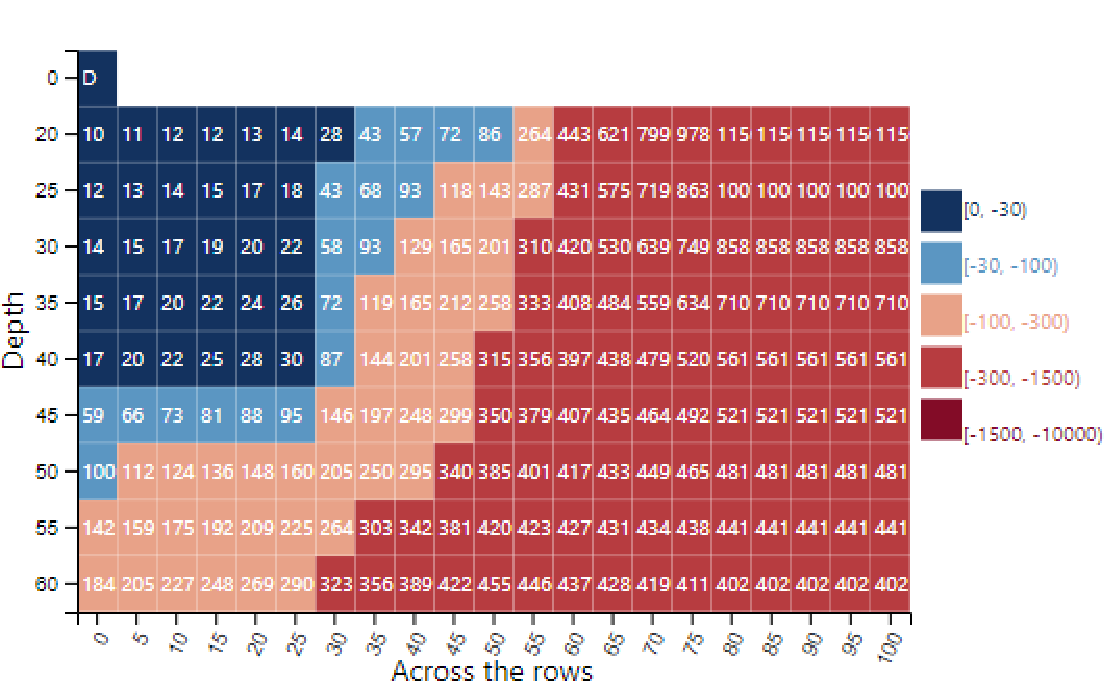
\includegraphics[width=\textwidth]{chapters/physics-aware/orchard/img/3gg_profile.pdf}
        \caption{3-days horizon}
        \label{orchard-fig:profile_c}
    \end{subfigure}
    \hfill
    \begin{subfigure}[b]{0.47\textwidth}
        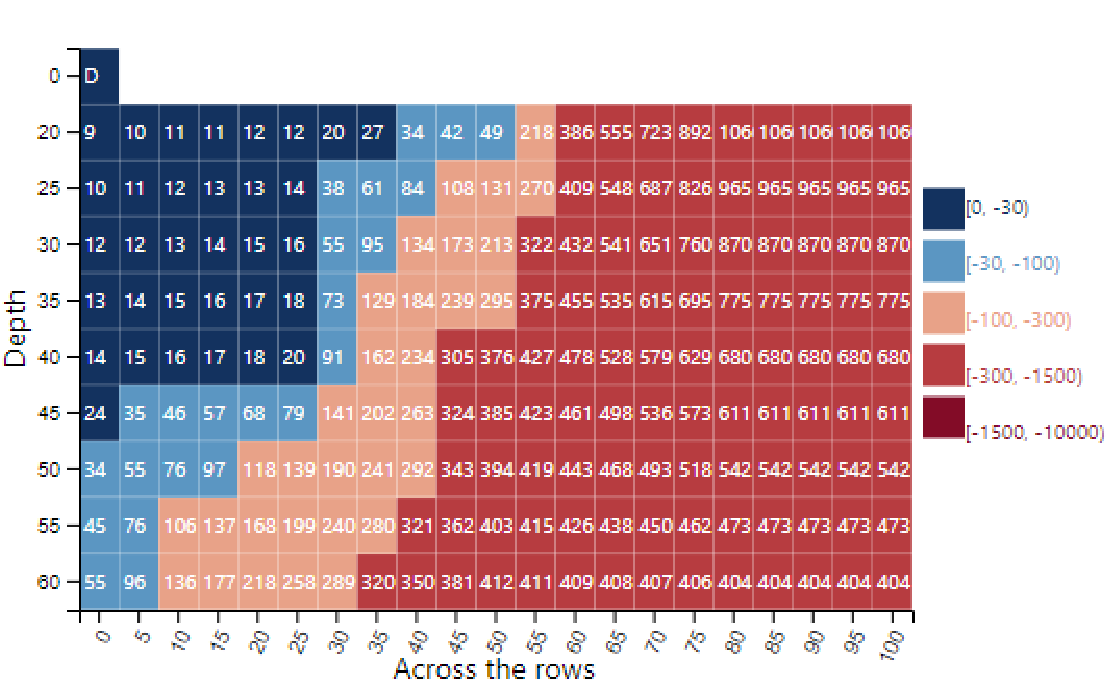
\includegraphics[width=\textwidth]{chapters/physics-aware/orchard/img/7gg_profile.pdf}
        \caption{7-days horizon}
        \label{orchard-fig:profile_d}
    \end{subfigure}
    \caption{2D-spatial soil moisture profiles.}
    \label{orchard-fig:profiles}
\end{figure}

\paragraph{Result Discussion} \Cref{orchard-fig:stacked} and \Cref{orchard-fig:profiles} shows a graphical representation of the measured soil moisture profile and compare it with the forecasting results. Colors emphasize water potential values according to five crop-specific soil moisture ranges (suggested by agronomist during the Agro.Big.Data.Science project \cite{ABDS}):
dark blue (in $[0, -30)$ cbar) and light blue (in $[-30, -100)$ cbar) show heavily/slightly portions of over-watered soil, salmon pink (in $[-100, -300)$ cbar) represents the ideal case \cite{miller1998effects}, while light red (in $[-300, -1500)$ cbar) and dark red (in the range of $[-1500, -10000)$ cbar) show slightly/heavily portions of under-watered soil.

While \Cref{orchard-fig:stacked} shows the soil moisture trend along the overall testing period, \Cref{orchard-fig:profiles} spatially details the profile on 10am July 26$^{th}$. The fine-grained spatial grid clearly shows how moisture changes depending on the dripper distance and according to the effect of the root system.
%
Forecasted profiles (sub-figures b,c,d) are very similar to the observed ones with slight differences appearing as the forecasting horizon increases.
\begin{figure}[!h]
    \centering
    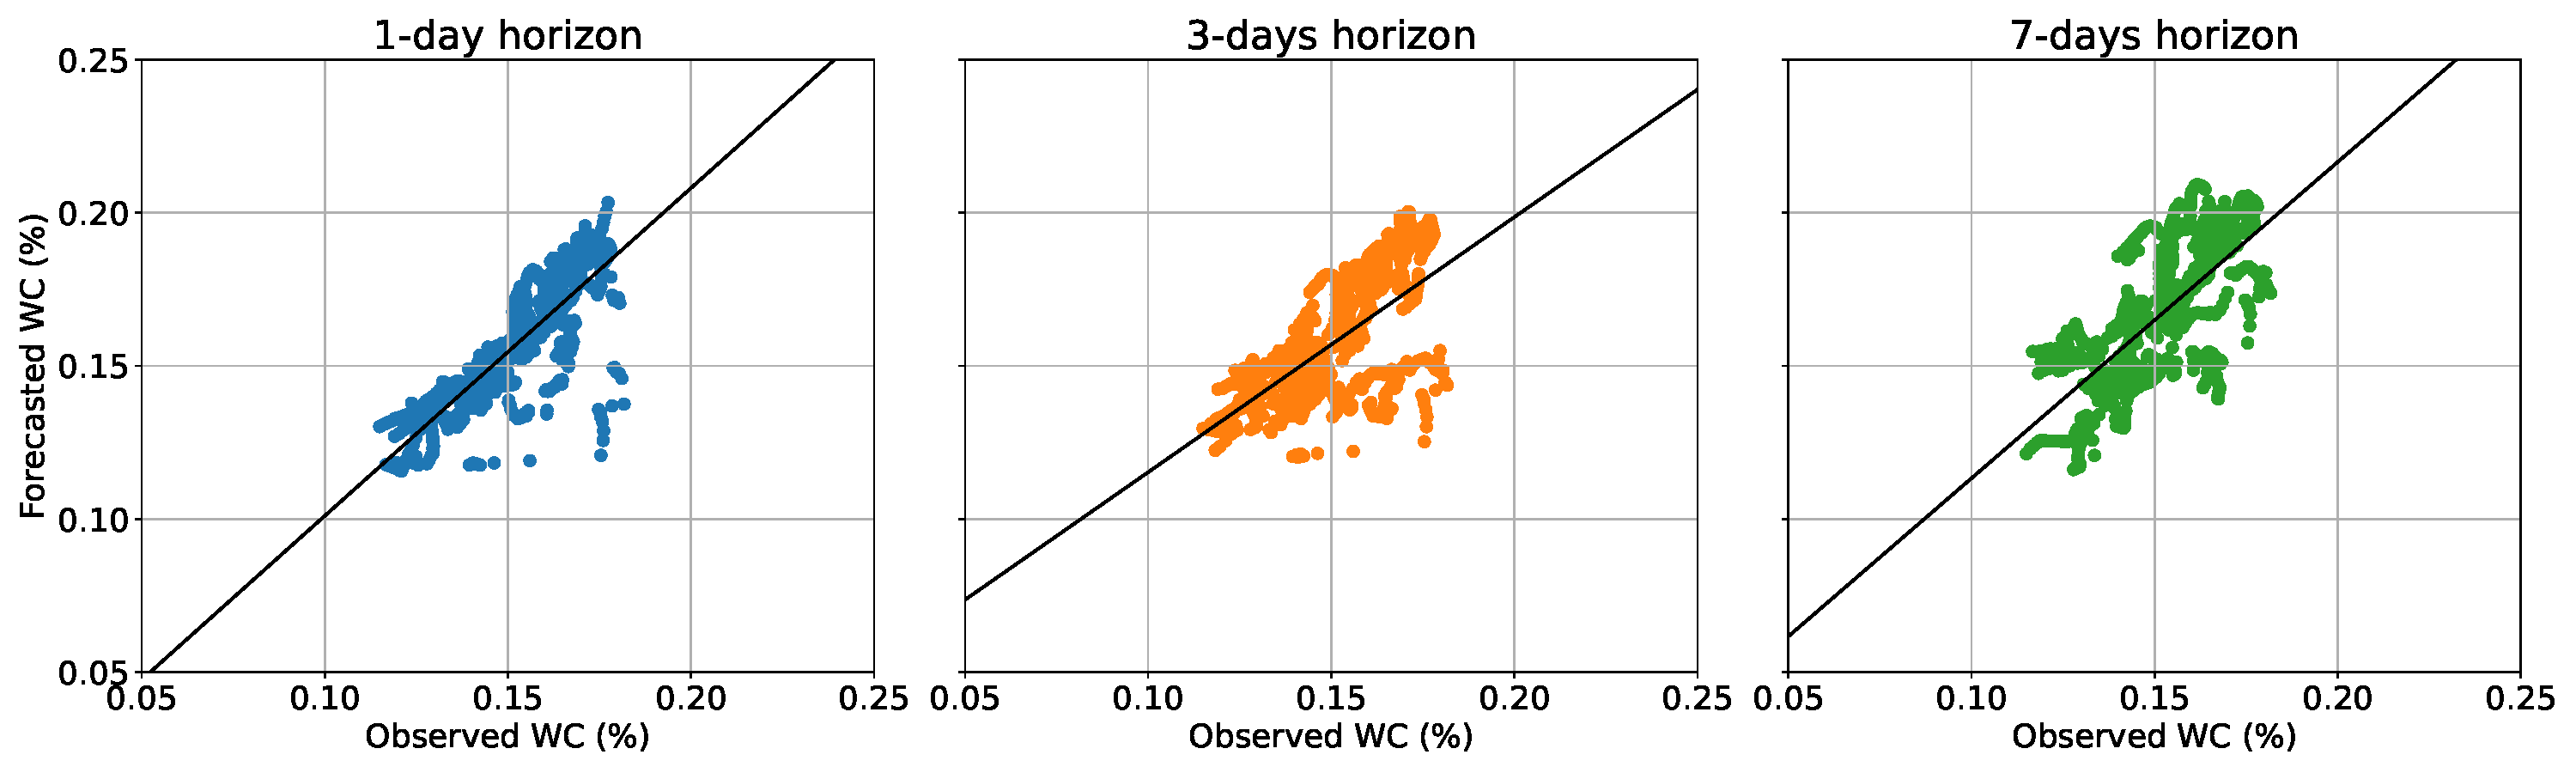
\includegraphics[scale=.27]{chapters/physics-aware/orchard/img/correlation_wc.pdf}
    \caption{Correlation between observed and forecasted  water content ($\%$).}
    \label{orchard-fig:scatter_correlation}
\end{figure}

Finally, \Cref{orchard-fig:scatter_correlation} reports a scatterplot showing the correlation between observed and forecasted water content.
%
The regression lines show the overall trend.
%
The more the forecasted values are close to the observed one, the less the regression line deviates from chart diagonal (i.e., the chart diagonal represent the full correlation between the two variables). Variables are well correlated on all the three time-horizons with best performance with 1-day forecast.
%
\olab{} tends to estimate the soil slightly over moistured in particular for high values of water content, while, for low values, \olab{} is extremely accurate.

\subsection{Parameter Tuning Performance}
\label{orchard-ssec:eval_tuner}

The parameter tuner is the data-driven process that automatically determines the right parameters for the current use case.
%
In this section, we verify the robustness of the procedure
%according to these two variables.
by considering 25\%, 50\%, and 75\% of the whole tuning period (June 21th - July 5th).
%
We evaluate the performance of the given sets of parameters as before: via the error metric (\Cref{orchard-eq:error}) when forecasting 1, 3, and 7 days ahead in the testing period (July 6th - August 31th).

\begin{table}[H]
\centering
\begin{tabular}{p{3cm}|ccc}
\toprule
Percentage of & \multicolumn{3}{c}{Forecasting horizon} \\
 tuning period & \multicolumn{1}{c|}{1 day} & \multicolumn{1}{c|}{3 days} & \multicolumn{1}{c}{7 days} \\ \midrule
25\%  & 0.27 ($\pm$ 0.14) & 0.47 ($\pm$ 0.25) & 0.56 ($\pm$ 0.29) \\
50\% & 0.25 ($\pm$ 0.14) & 0.41 ($\pm$ 0.23) & 0.59 ($\pm$ 0.24) \\
75\% & 0.27 ($\pm$ 0.15) & 0.45 ($\pm$ 0.23) & 0.63 ($\pm$ 0.22) \\
100\% & 0.27 ($\pm$ 0.13) & 0.43 ($\pm$ 0.22) & 0.55 ($\pm$ 0.24) \\ \bottomrule
\end{tabular}

\caption{Error (\Cref{orchard-eq:error}) and standard deviation considering different portions of tuning period.}
\label{orchard-tbl:tuning_budget}
\end{table}

\Cref{orchard-tbl:tuning_budget} shows the results. As a general trend, errors slightly decrease when more tuning data are available for every forecasting horizons. More data translates into more hydraulic dynamic examples, which are useful to better estimate the parameters, and hence make the forecasts more reliable.
Although the general trend, \olab{} is able to achieve good performance even with 25\% and 50\% of the considered period.
Above all, the case of 50\% does not consider the rain in the beginning of June (which brings some fluctuations in the calculus) and achieves excellent performance.
The standard deviation remains steady along the forecasting horizon.
Overall, the insights suggest that the tuning phase of \olab{} is robust in suggesting soil and plant parameters for the use-case at hand.


\section{Conclusions and Future Works}
In this chapter, we proposed an integrated system coupling a three dimensional crop model with a assimilation procedure that exploit a bi-dimensional sensor grid. Forecasted soil moisture data up to a 7 day horizon has proven to be precise enough to support precision watering. Testing has been carried out on a real kiwi-fruit orchard. The real-data sensor are also used to carry out the auto-tuning of the soil parameter in order to achieve a field specific forecast. Robustness tests emphasized that few days of hourly samples are enough to properly set the field parameters. This make our approach practically applicable. 

We are now working towards closing the loop and creating a prescriptive system delivering a watering advice. \olab{} will be exploited to forecast the combined effects of weather conditions and watering policies to return the watering advice that fits at best an optimal soil moisture profile.  Working on a 7 days period, we can handle complex cases were constraints (e.g. water availability) do not allow daily irrigation.
